\documentclass{beamer}
\usepackage{ctex, hyperref}

% other packages
\usepackage{latexsym,amsmath,xcolor,multicol,booktabs,calligra}
\usepackage{graphicx,pstricks,listings,stackengine}
\usepackage{tsinghua}
\usepackage{subcaption}
\usepackage{siunitx}
\usepackage{physics}
\usepackage{bm}

\title{基于物理模拟的正颌手术术后外形预测}
\subtitle{毕业设计中期汇报}
\author{李钦 \\ 指导教师: 徐枫}
\institute{清华大学软件学院}
\date{2024 年 4 月 7 日}

\DeclareMathOperator{\dist}{dist}

\begin{document}

\kaishu

\begin{frame}
  \titlepage
\end{frame}

\begin{frame}
  \tableofcontents[sectionstyle=show,subsectionstyle=show/shaded/hide,subsubsectionstyle=show/shaded/hide]
\end{frame}

\section{研究问题}

\begin{frame}{研究问题}
  \begin{description}
    \item[应用场景] 正颌手术规划中, 预测术后患者的面部外形
    \item[输入] 术前患者的头部 CT 数据, 术后患者的颅骨模型
    \item[输出] 术后患者的面部模型
    \item[数据] 多组术前, 术后的患者 CT 数据
  \end{description}
\end{frame}

\section{三维医学模型重建}

\begin{frame}{三维医学模型重建}
  \begin{description}
    \item[目标] CT (voxel grid) $\to$ tetrahedral mesh
    \item[步骤]
          \begin{enumerate}
            \item 构建 template mesh
            \item 预处理 CT 数据
            \item rigid alignment
            \item non-rigid registration
            \item 使用 TetGen 进行 tessellation
          \end{enumerate}
  \end{description}
  \begin{figure}
    \centering
    \subcaptionbox{CT}{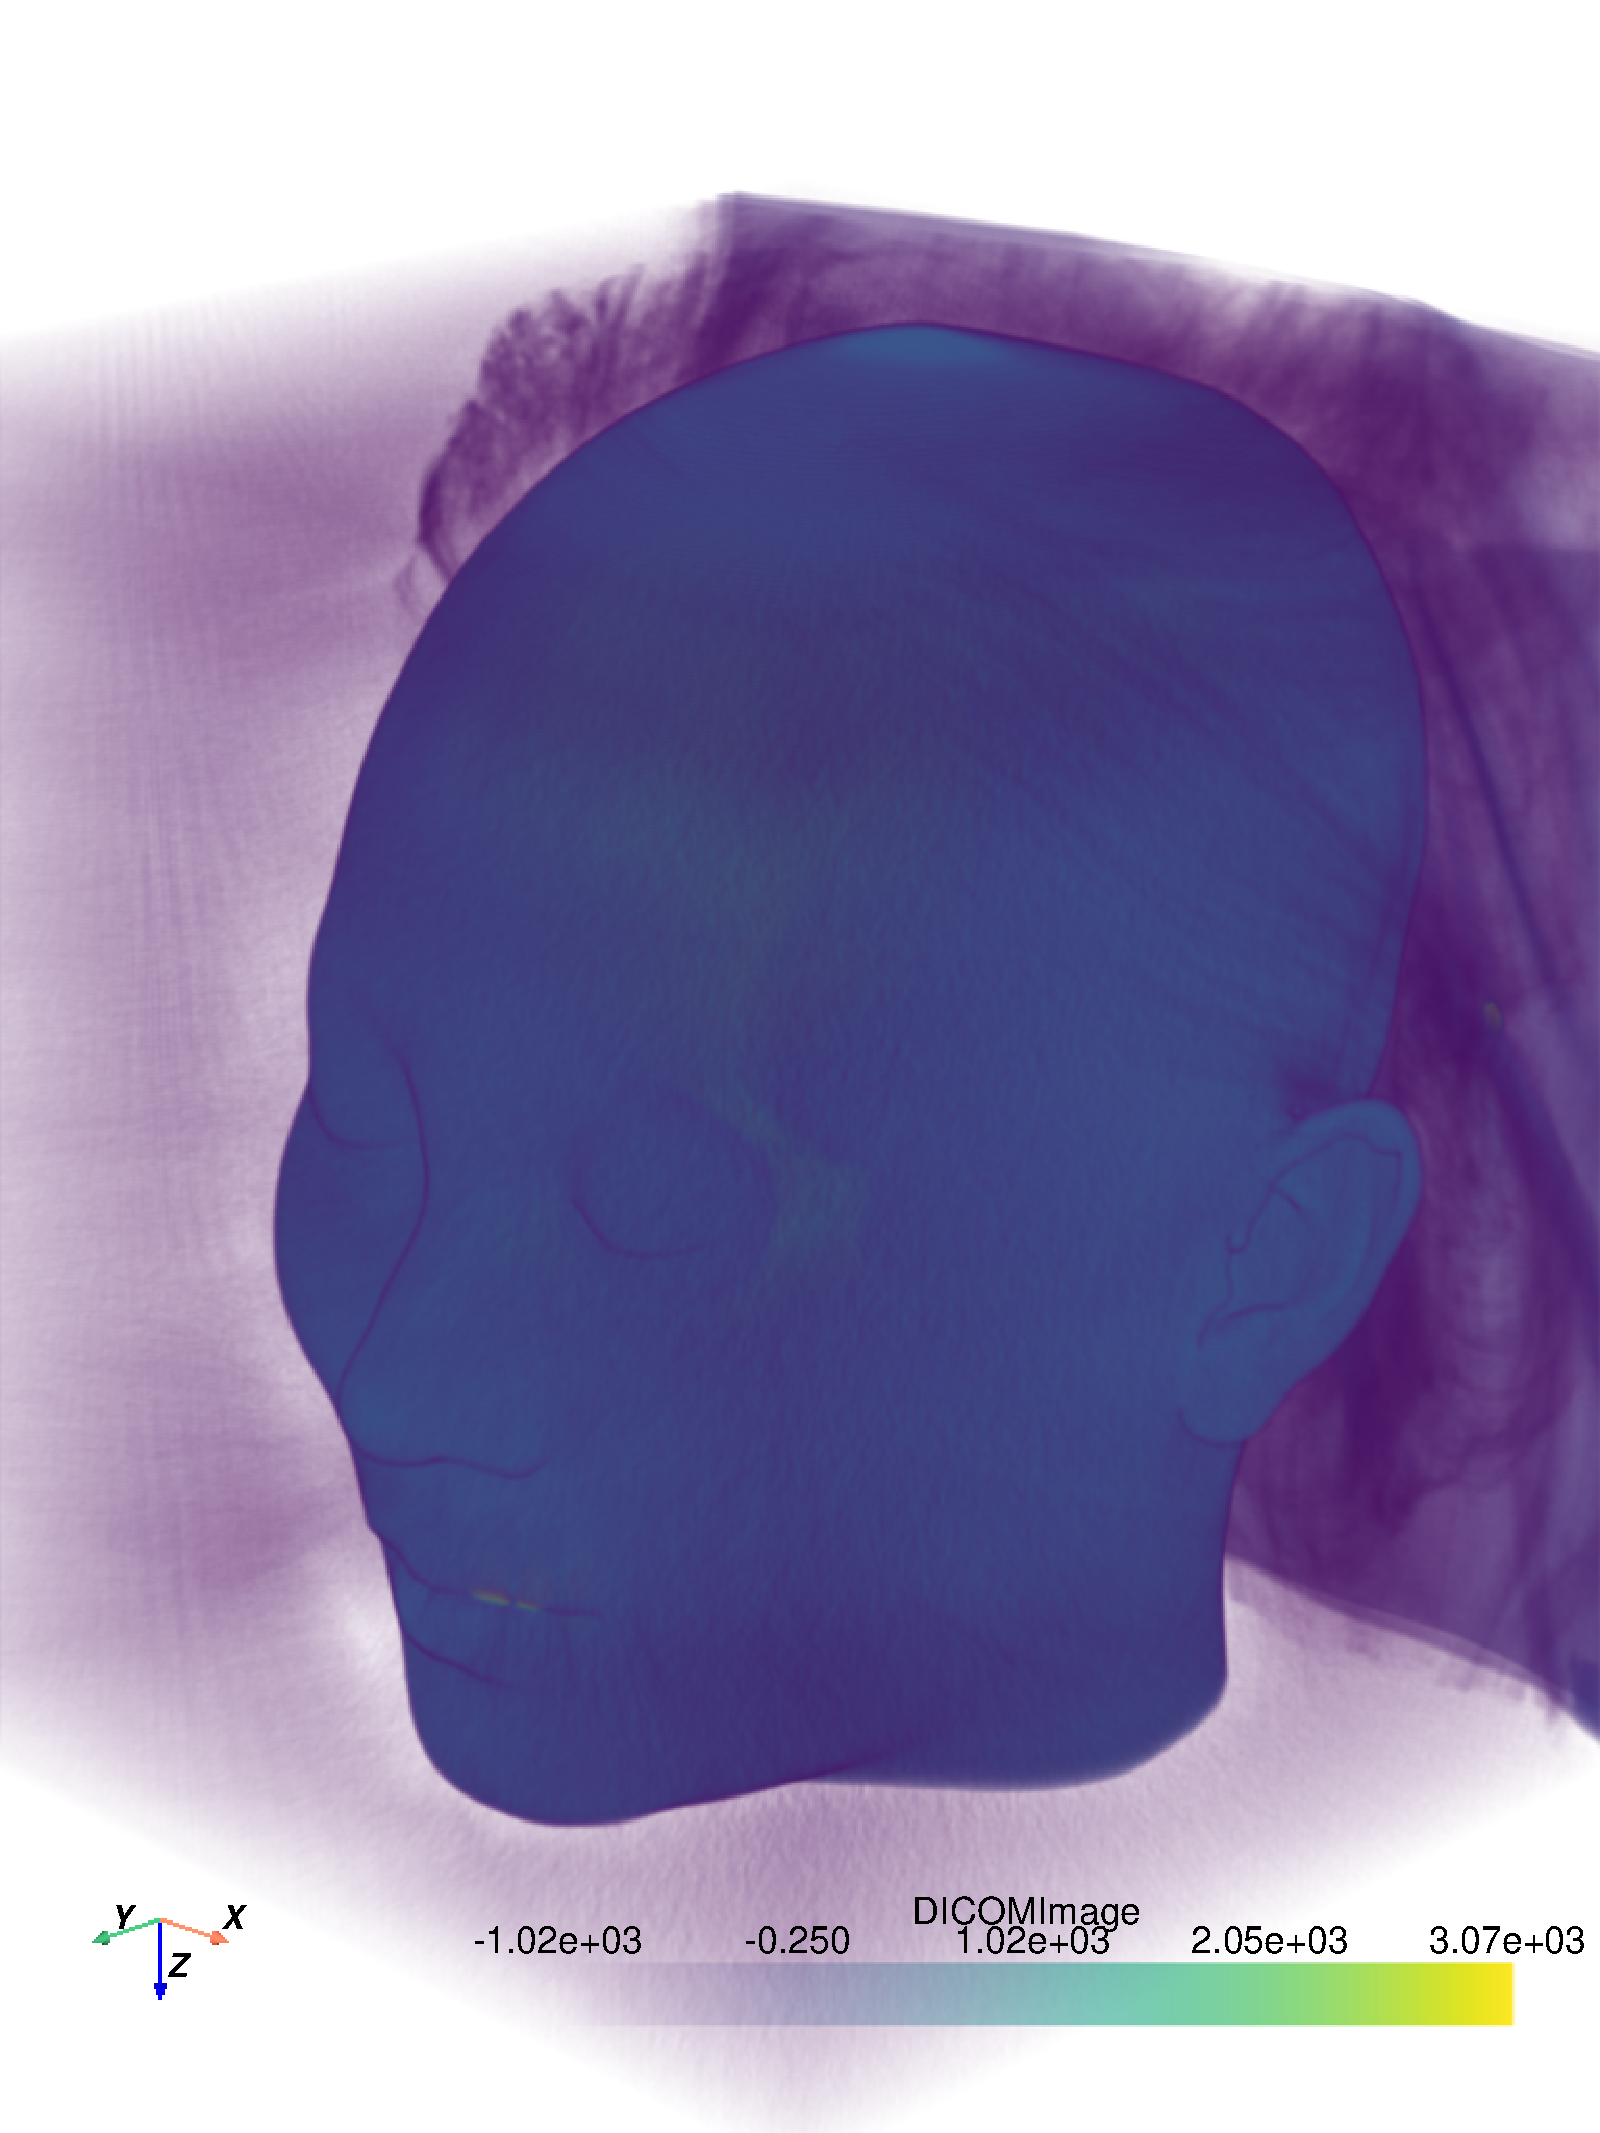
\includegraphics[height = 0.4 \linewidth]{fig/CT.pdf}}
    \subcaptionbox{Tetrahedral Mesh}{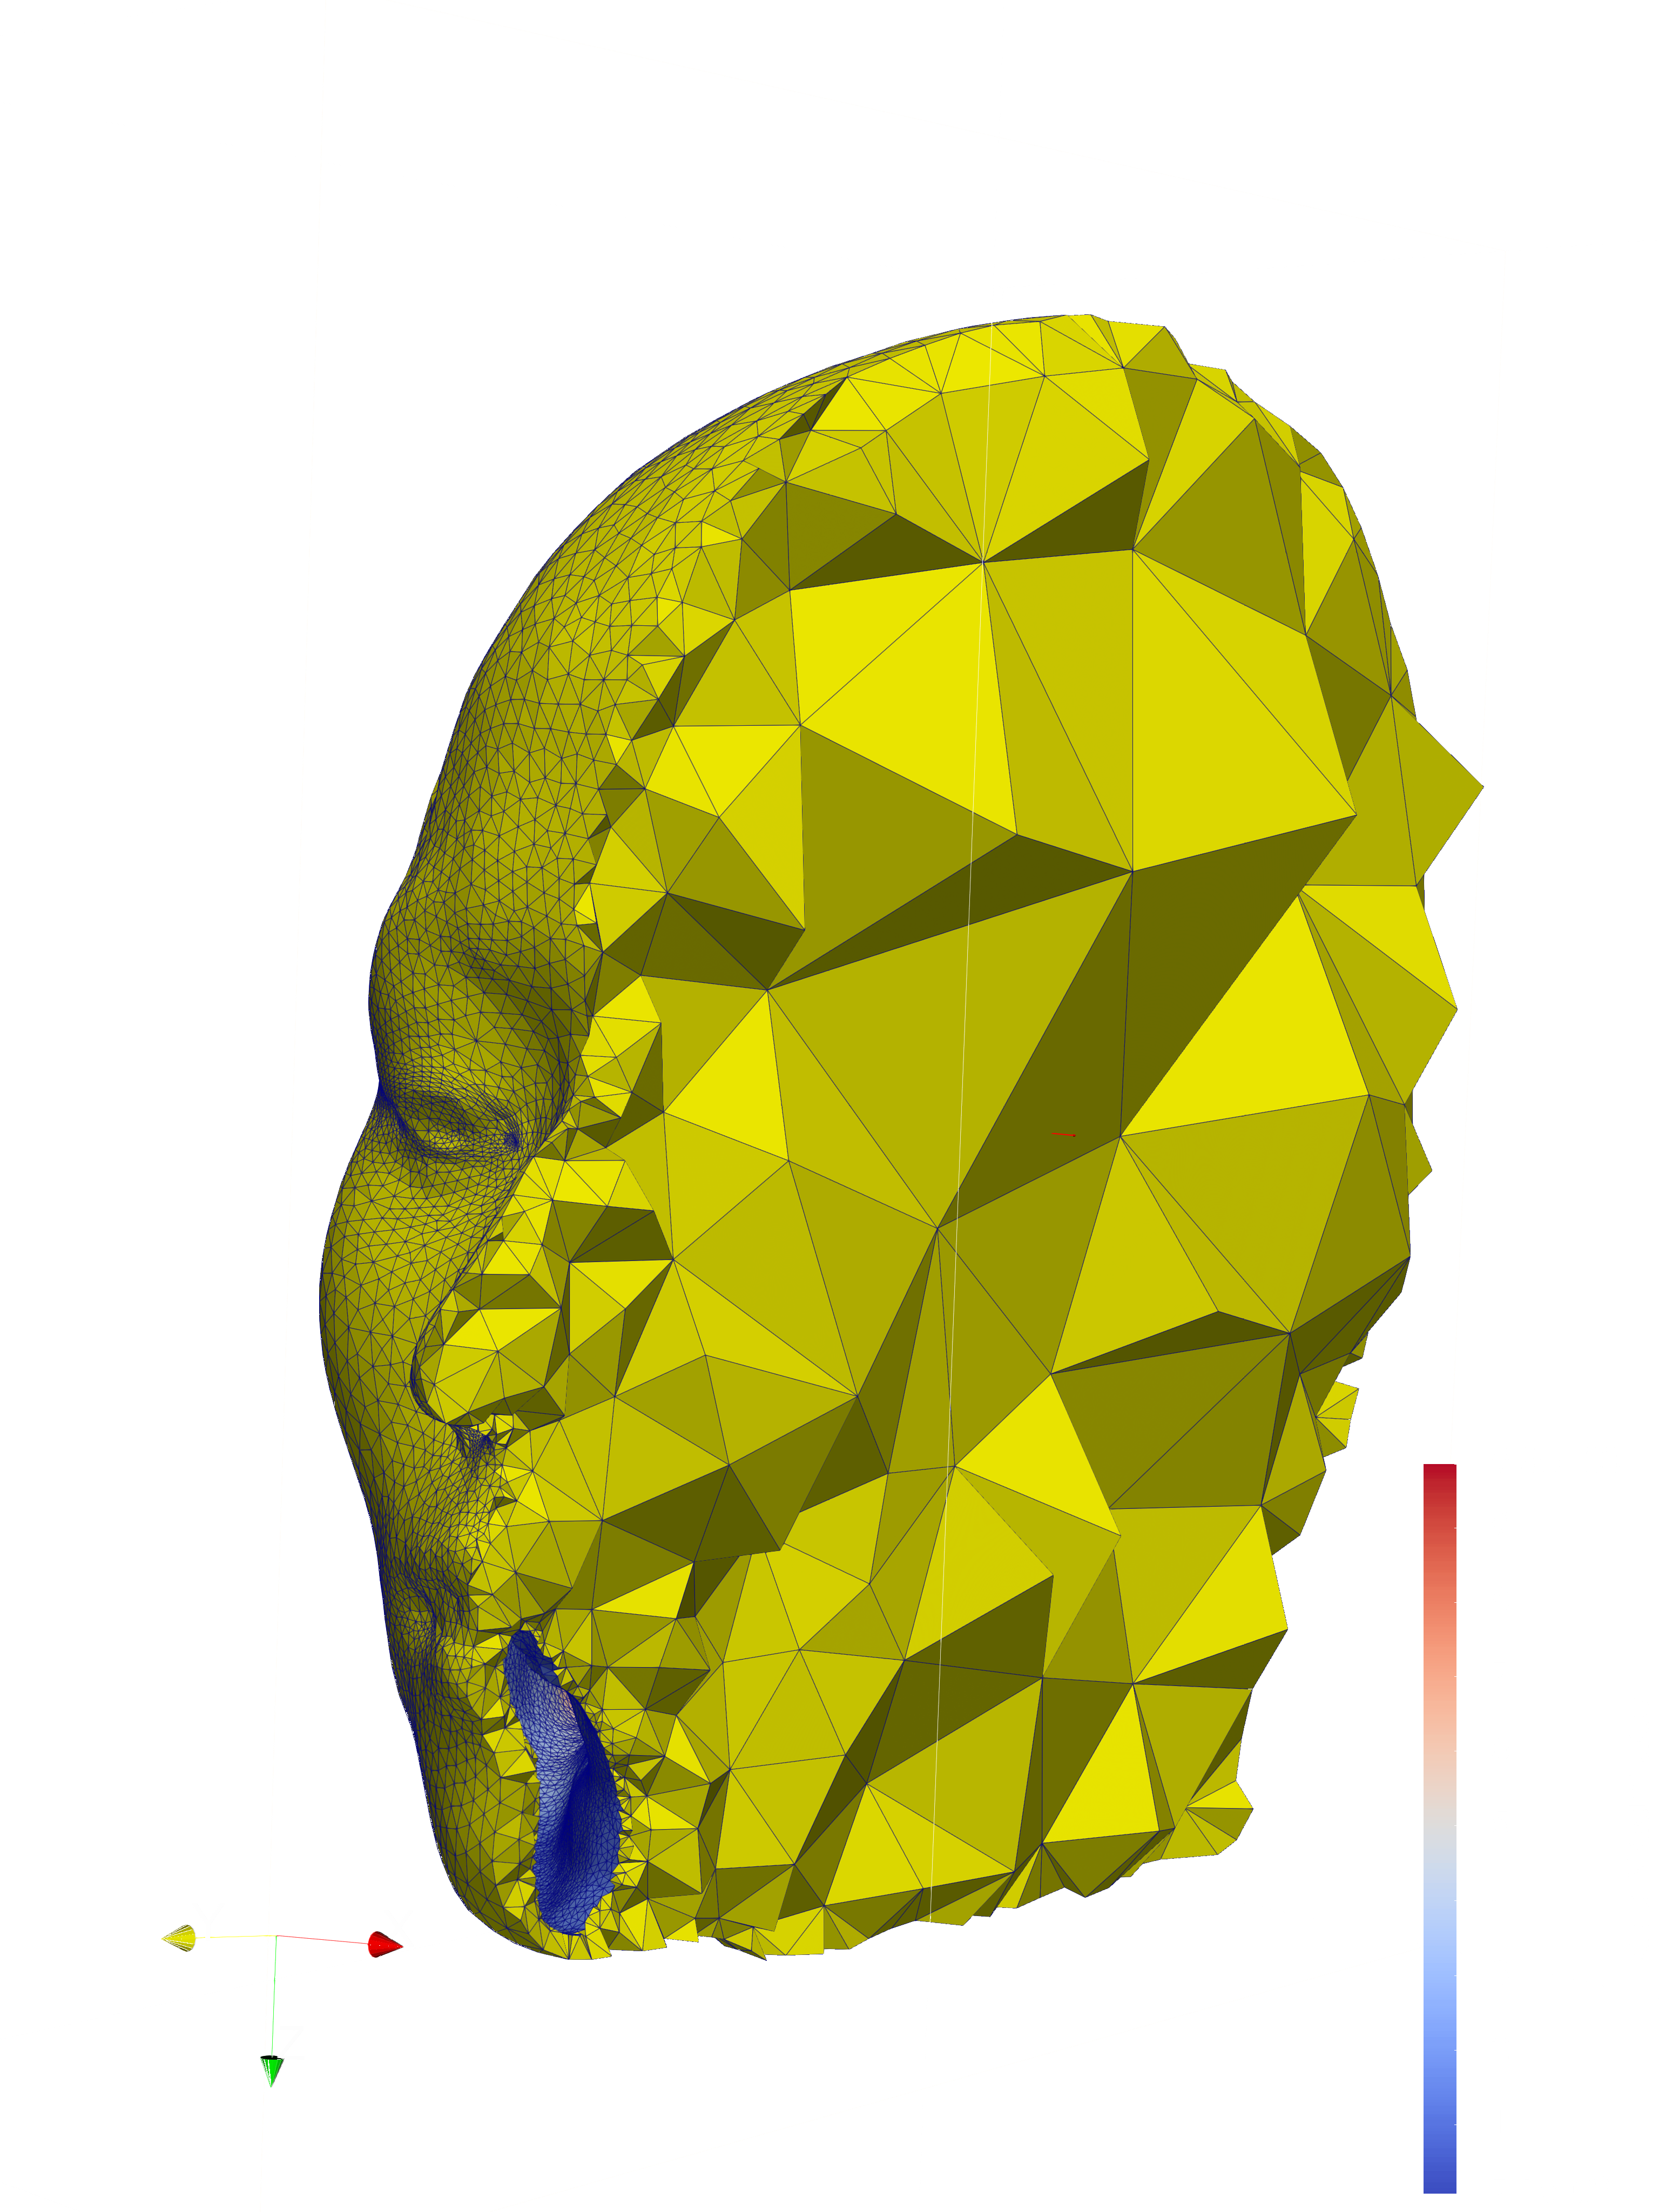
\includegraphics[height = 0.4 \linewidth]{fig/tet.png}}
  \end{figure}
\end{frame}

\begin{frame}{构建 Template Mesh}
  \begin{enumerate}
    \item 基于 SCULPTOR 开源的 template mesh 构建
    \item 移除内部结构, 如: 嘴唇向内延伸的部分
    \item 删去 CT 中不包含的部分, 如: 大部分的颈部和肩部
    \item 使用 MeshFix 填补孔洞, 如: 眼睛, 嘴, 颈
    \item Laplacian smoothing \& taubin filtering
  \end{enumerate}
  \begin{figure}
    \centering
    \subcaptionbox{Original Template Face}{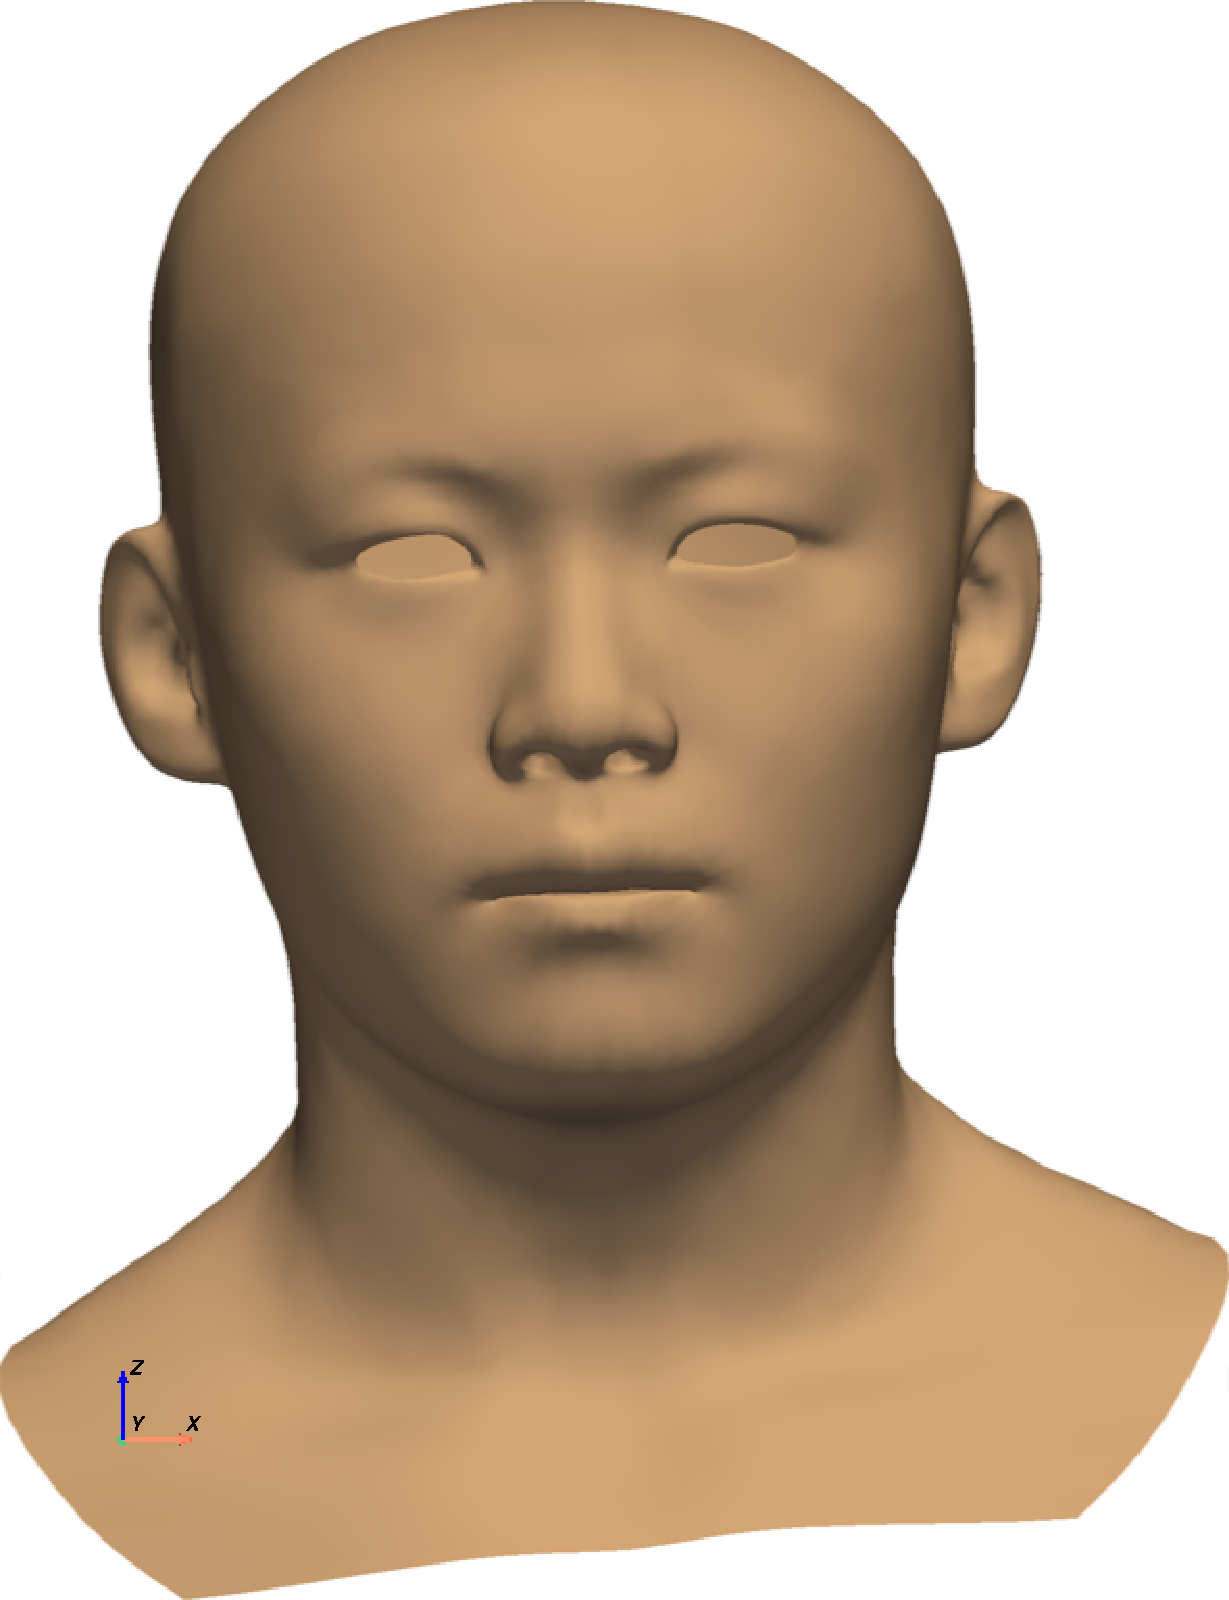
\includegraphics[height = 0.4 \linewidth]{fig/template-face-00.pdf}}
    \subcaptionbox{Modified Template Face}{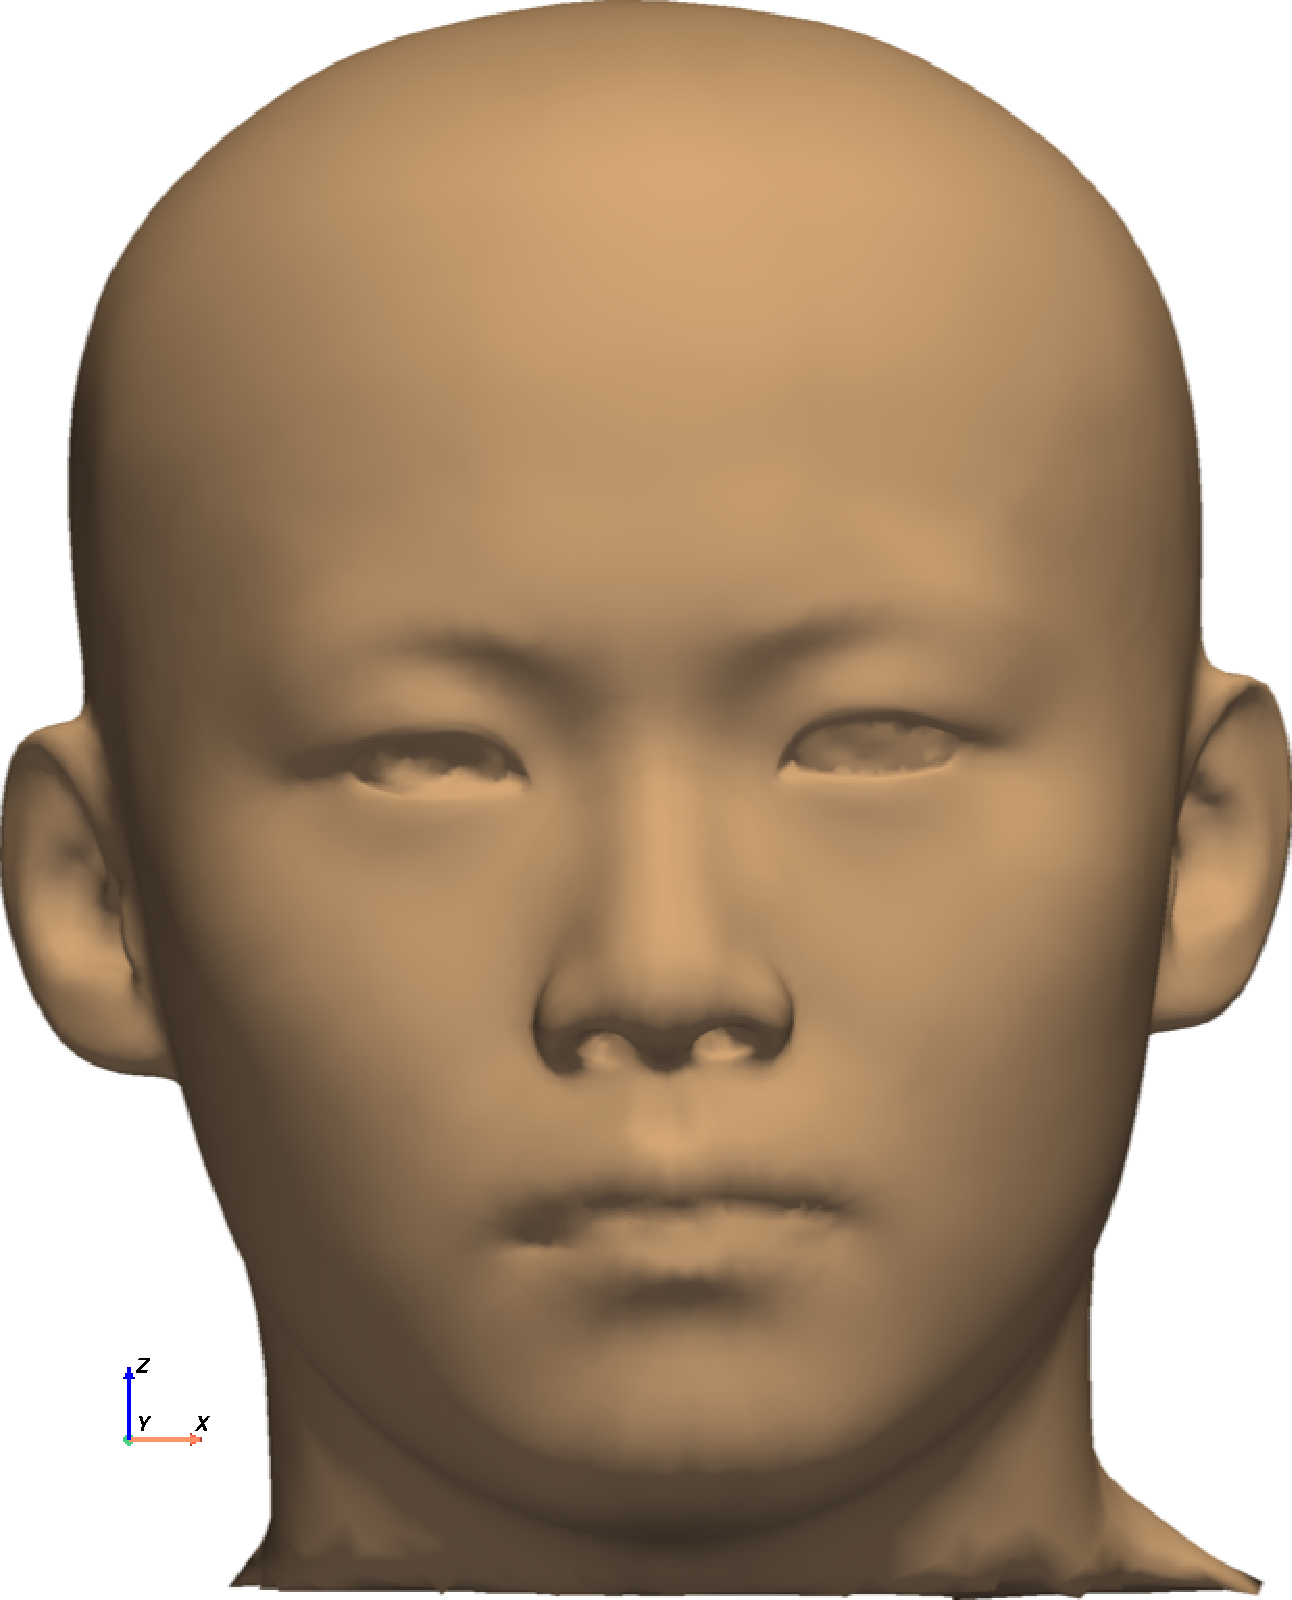
\includegraphics[height = 0.4 \linewidth]{fig/template-face-01.pdf}}
  \end{figure}
\end{frame}

\begin{frame}{Rigid Alignment}
  \textcolor{tsinghua}{目标} 从 CT 数据提取表面 mesh, 将 template mesh 变换至与之对齐
  \begin{enumerate}
    \item 对 CT 做 Gaussian smoothing
    \item 对 CT 使用 VTK contour filter 根据阈值 (骨骼取 \num{128}, 软组织取 \num{-128}) 分割, 得到 isosurface, 即 target mesh
    \item 在 template mesh 和 target mesh 上人工标注 landmarks, 由 Procrustes' analysis 得到全局刚性变换 (平移 + 缩放 + 旋转)
    \item ICP (Iterative Closest Point) 优化刚性变换
  \end{enumerate}
\end{frame}

\begin{frame}{CT to Mesh}
  \begin{figure}
    \centering
    \subcaptionbox{CT}{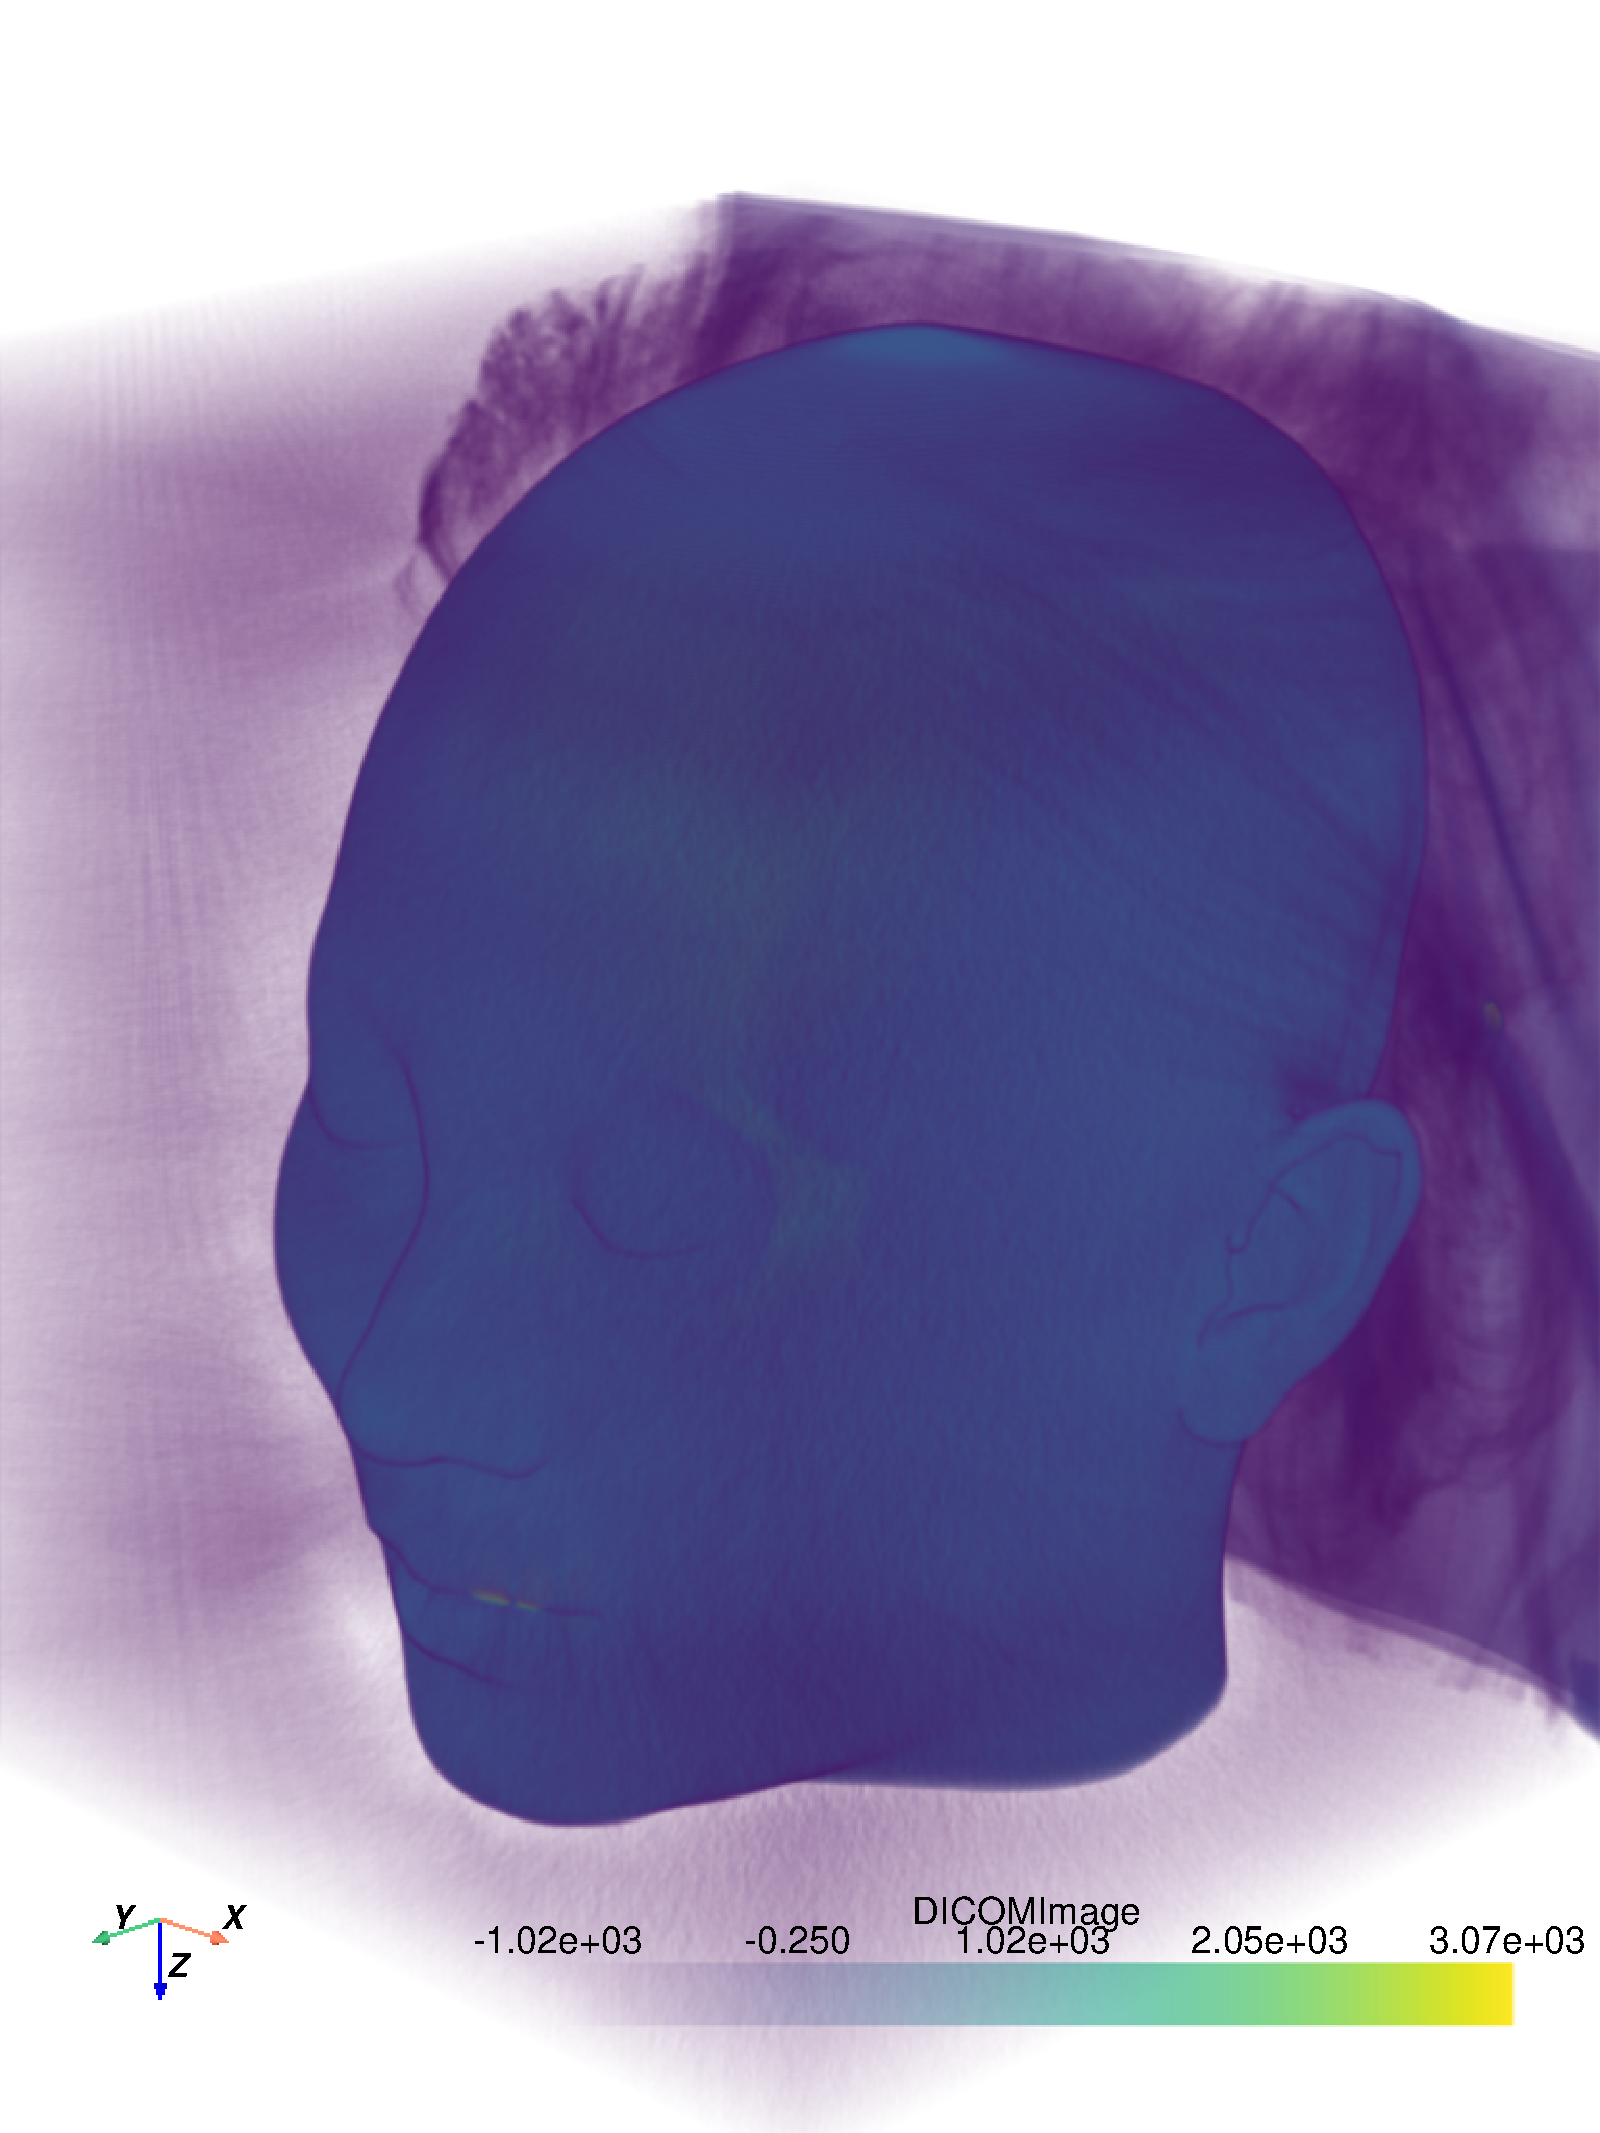
\includegraphics[width = 0.3 \linewidth]{fig/CT.pdf}}
    \subcaptionbox{Face}{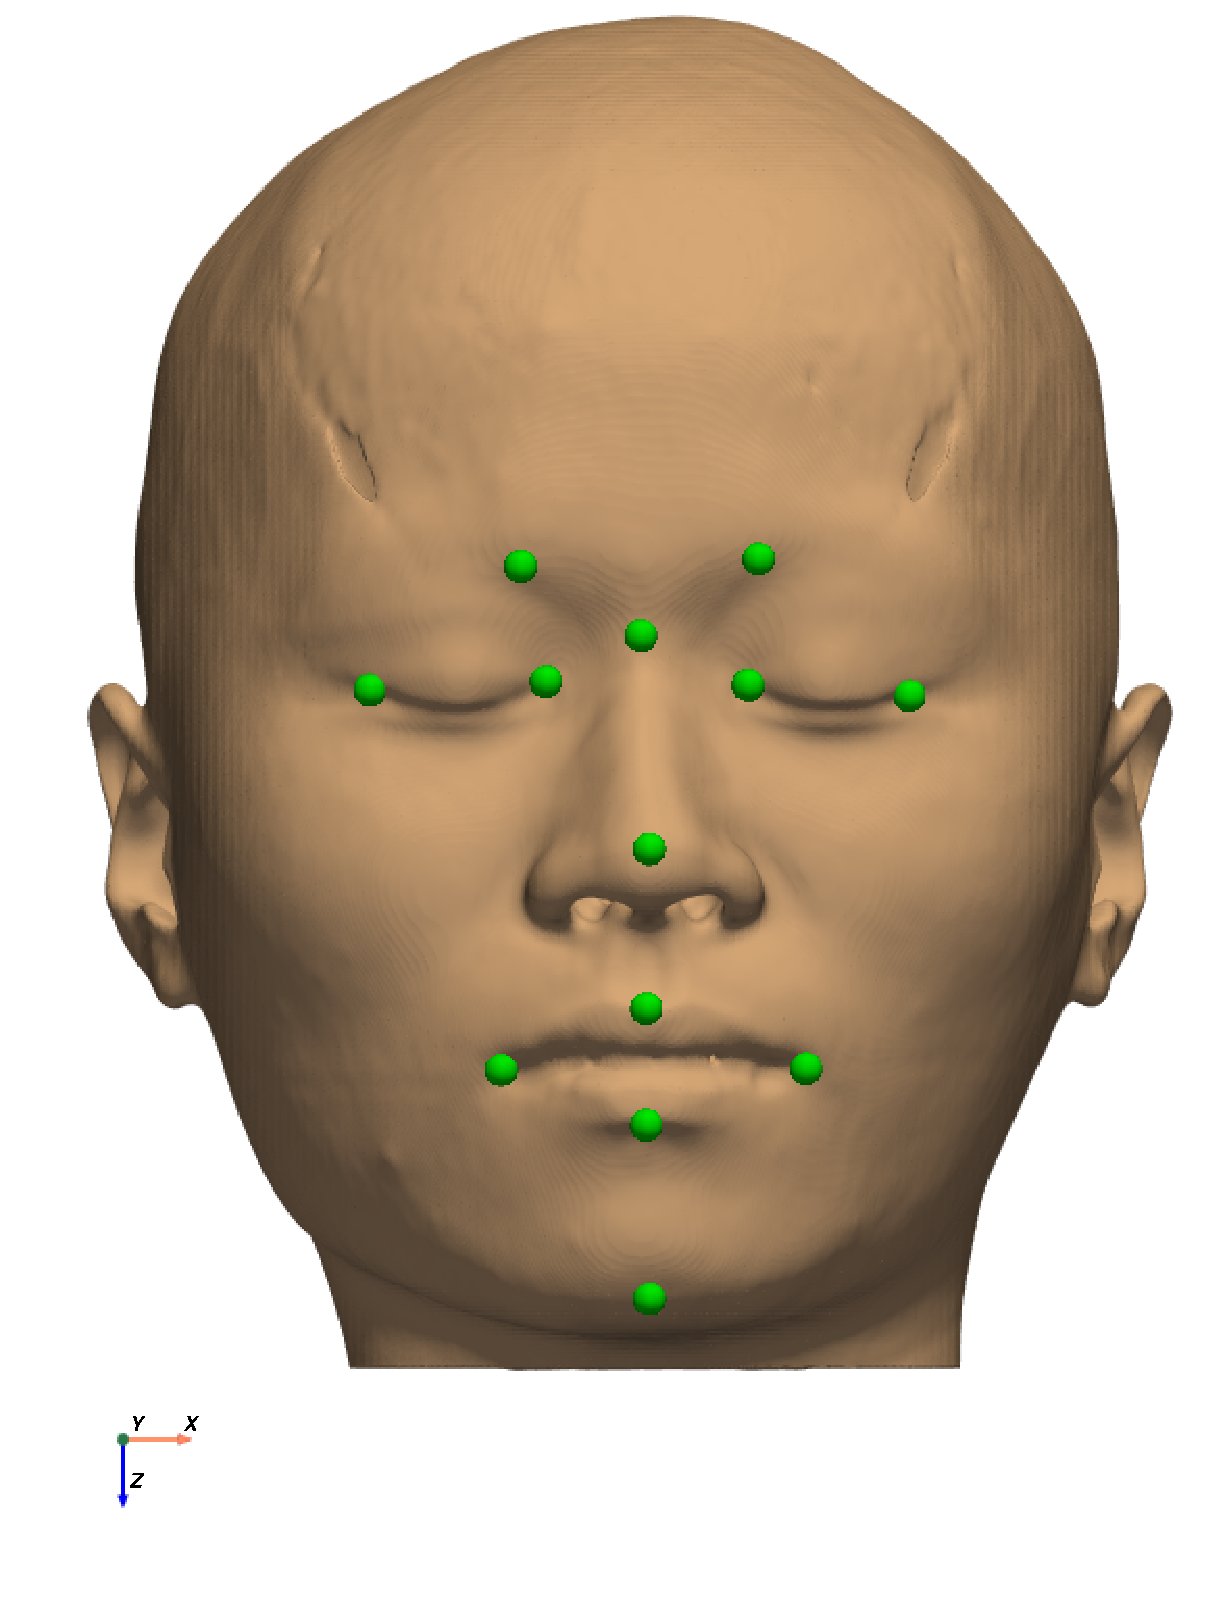
\includegraphics[width = 0.3 \linewidth]{fig/target-face-front.pdf}}
    \subcaptionbox{Skull}{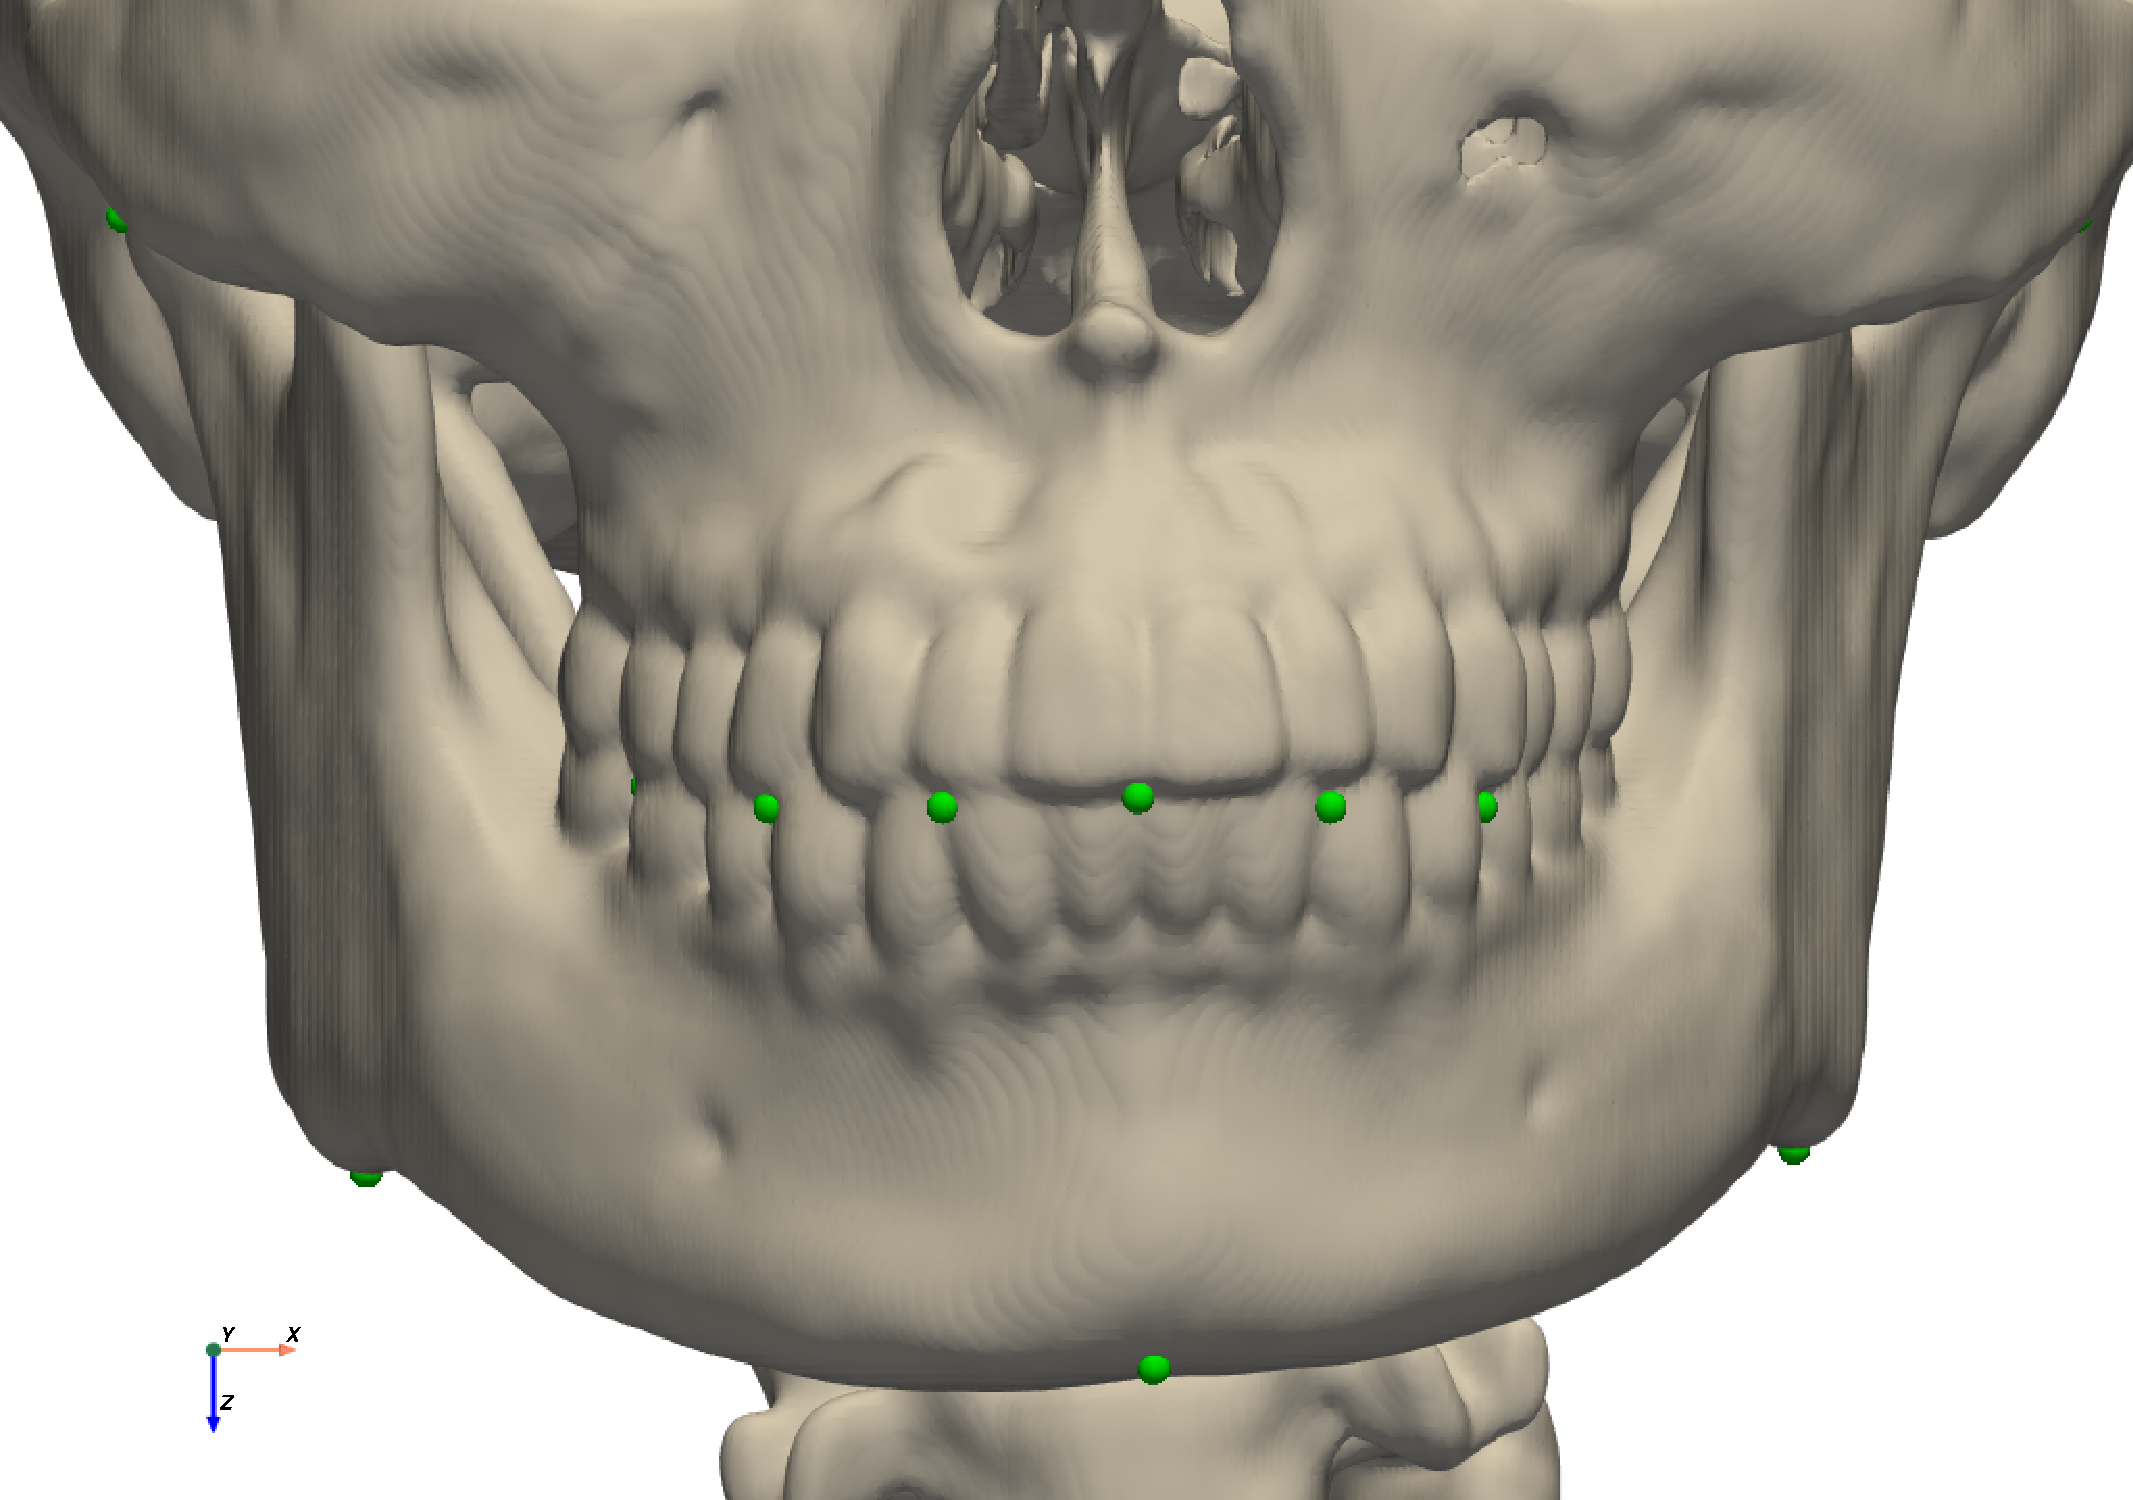
\includegraphics[width = 0.3 \linewidth]{fig/target-skull-front.pdf}}
  \end{figure}
\end{frame}

\begin{frame}{Non-rigid Registration}
  \textcolor{tsinghua}{目标} 将 template mesh 变形至与 target mesh 一致
  \begin{enumerate}
    \item 初始化 template mesh 和 target mesh 有效区域 $\mathcal{S}_v, \mathcal{T}_v$
    \item 对于每一组超参数
          \begin{enumerate}
            \item 初始化对应关系
                  \begin{equation*}
                    \mathrm{NN}(\bm{v}_i) = \arg\min_{\bm{u}_j \in \mathcal{T}_v} \norm{\bm{v}_i - \bm{u}_j} + \nu \norm{\bm{n}_{\bm{v}_i} - \bm{n}_{\bm{u}_j}}^2
                  \end{equation*}
            \item 最小化损失函数 $E = E_d + \alpha E_s + \beta E_l$
                  \begin{align*}
                    \text{distance} \quad E_d(\mathcal{X})  & = \sum_{\bm{v}_i \in \mathcal{S}_v} \dist^2(\mathcal{T}_v, \bm{X}_i \bm{v}_i) + \sum_{\bm{u}_i \in \mathcal{T}_v} \dist^2(\mathcal{X} \mathcal{S}_v, \bm{u}_i) \\
                    \text{stiffness} \quad E_s(\mathcal{X}) & = \sum_{(\bm{v}_i, \bm{v}_j) \in \mathcal{E}} \norm{(\bm{X}_i - \bm{X}_j) \bm{G}}_F^2                                                                          \\
                    \text{landmarks} \quad E_l(\mathcal{X}) & = \sum_{(\bm{l}_i, \bm{v}_i) \in \mathcal{L}} \dist^2(\bm{l}_i, \bm{X}_i \bm{v}_i)
                  \end{align*}
          \end{enumerate}
  \end{enumerate}
\end{frame}

\begin{frame}{Non-rigid Registration}
  \begin{table}
    \centering
    \begin{tabular}{ccc}
      Template                                                              & Patient                                                               & Result                                                                \\
      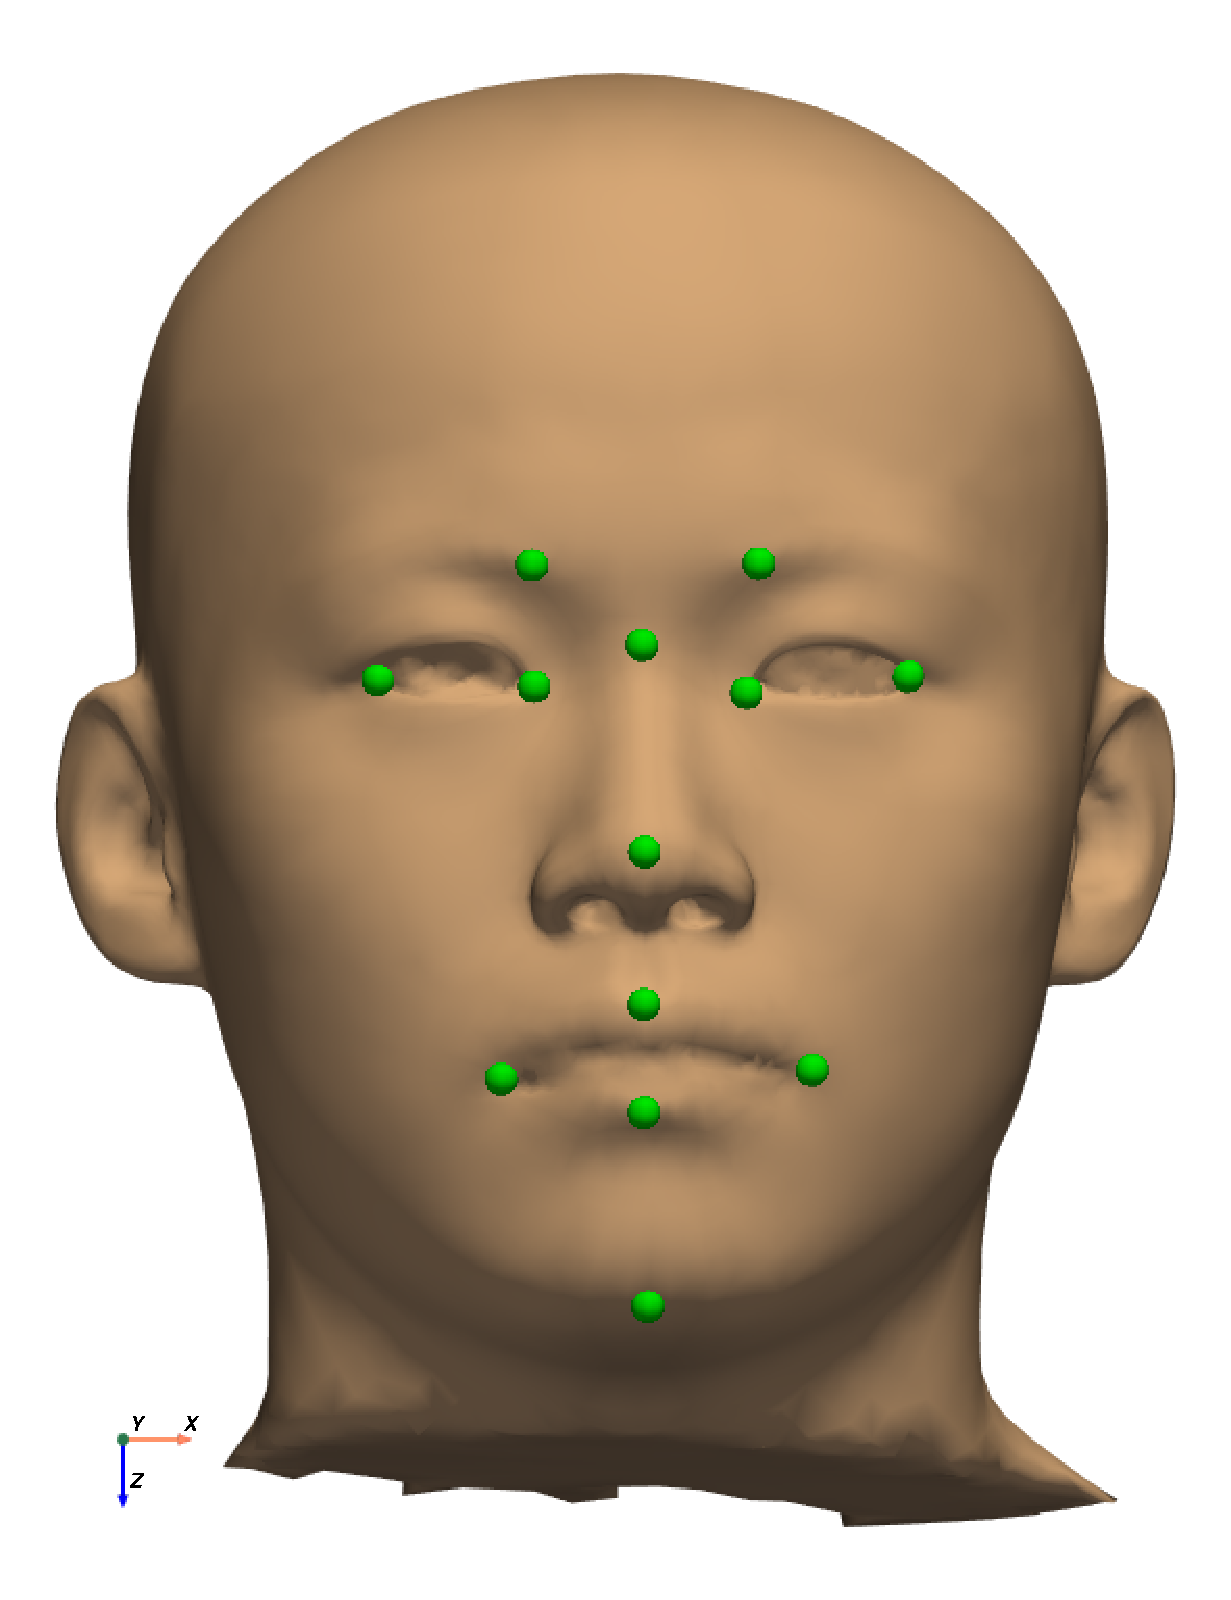
\includegraphics[height = 0.29 \linewidth]{fig/source-face-front.pdf} & 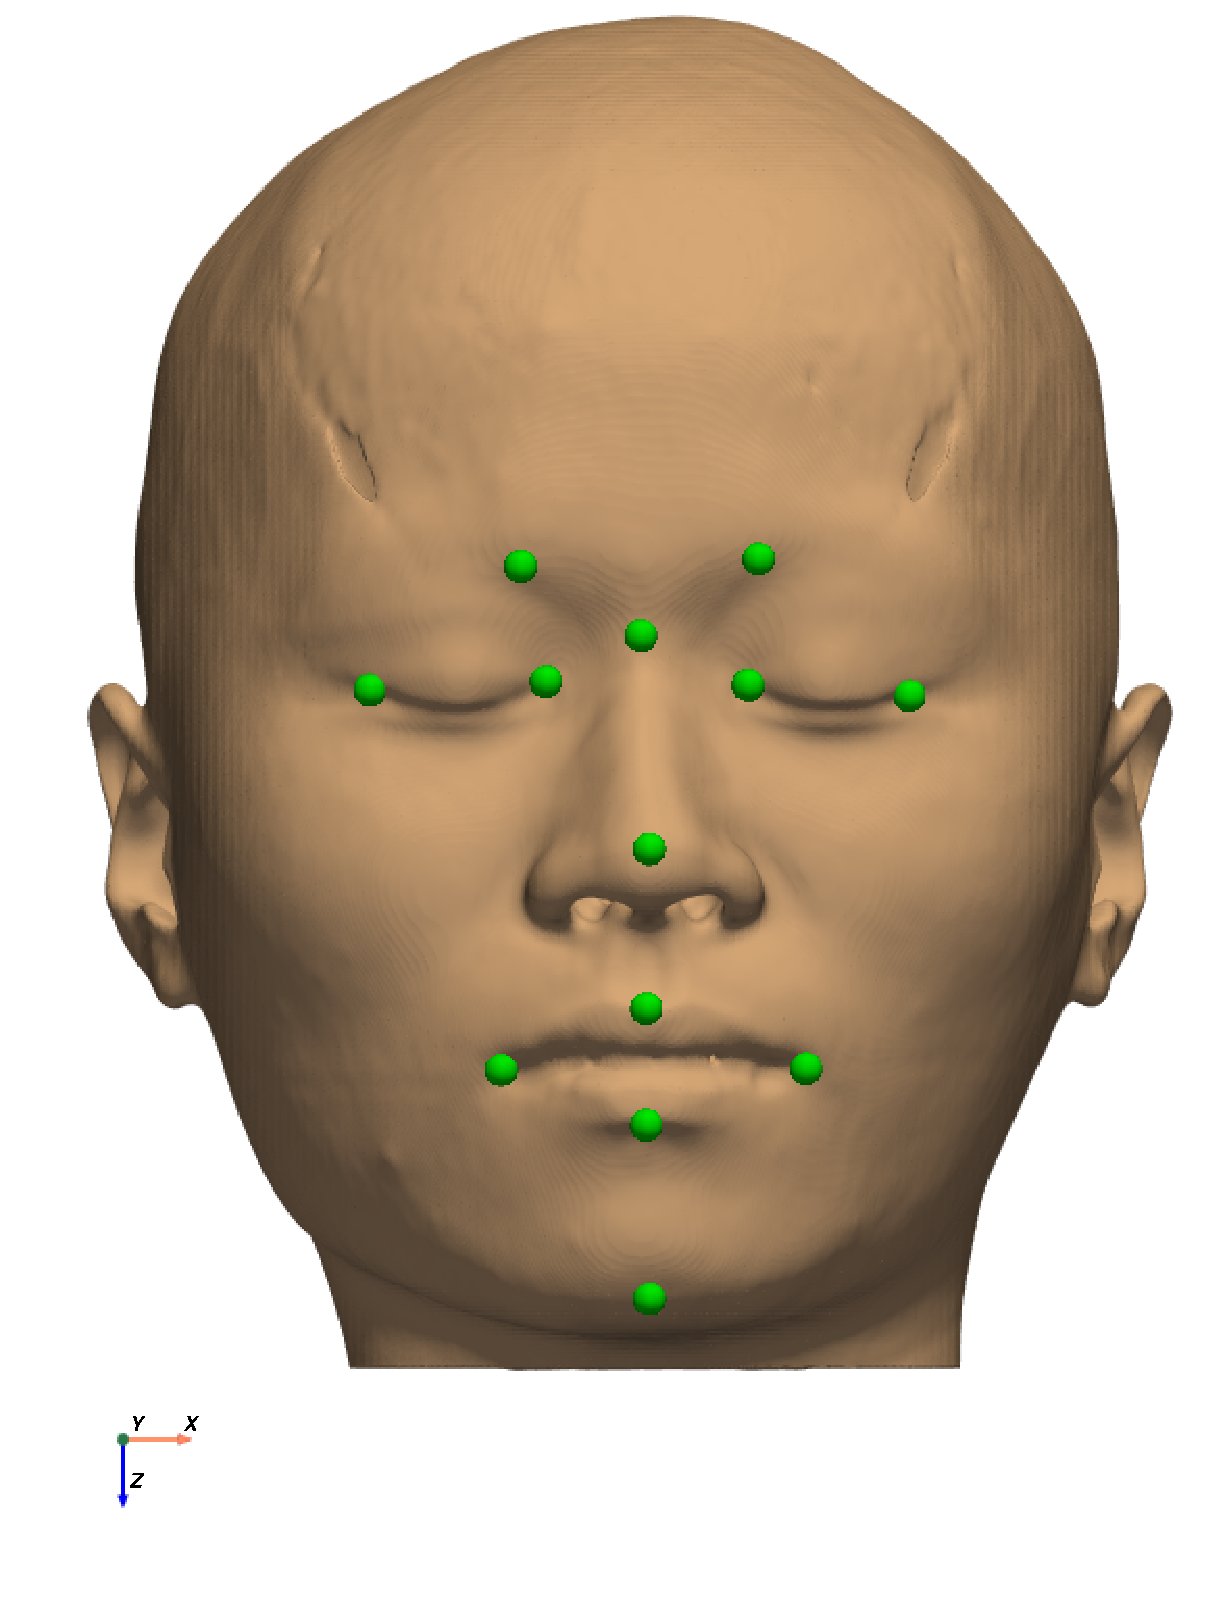
\includegraphics[height = 0.29 \linewidth]{fig/target-face-front.pdf} & 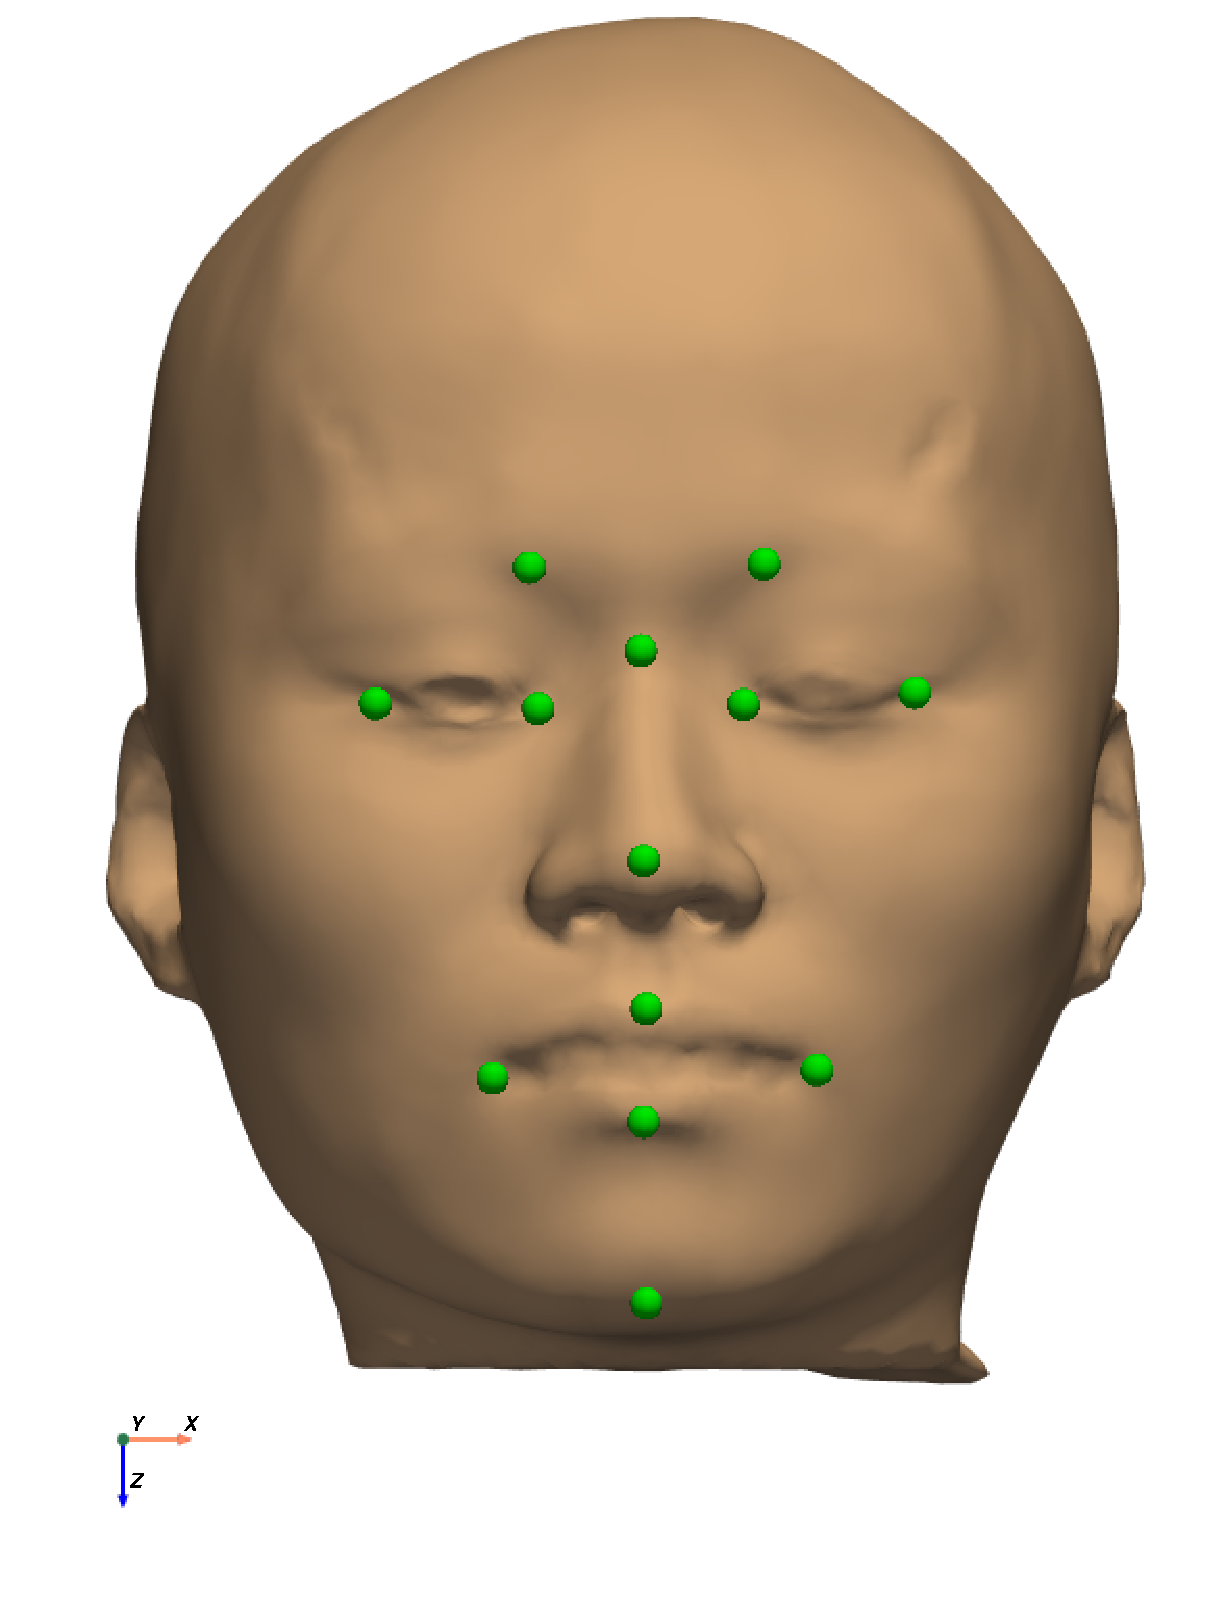
\includegraphics[height = 0.29 \linewidth]{fig/result-face-front.pdf} \\
      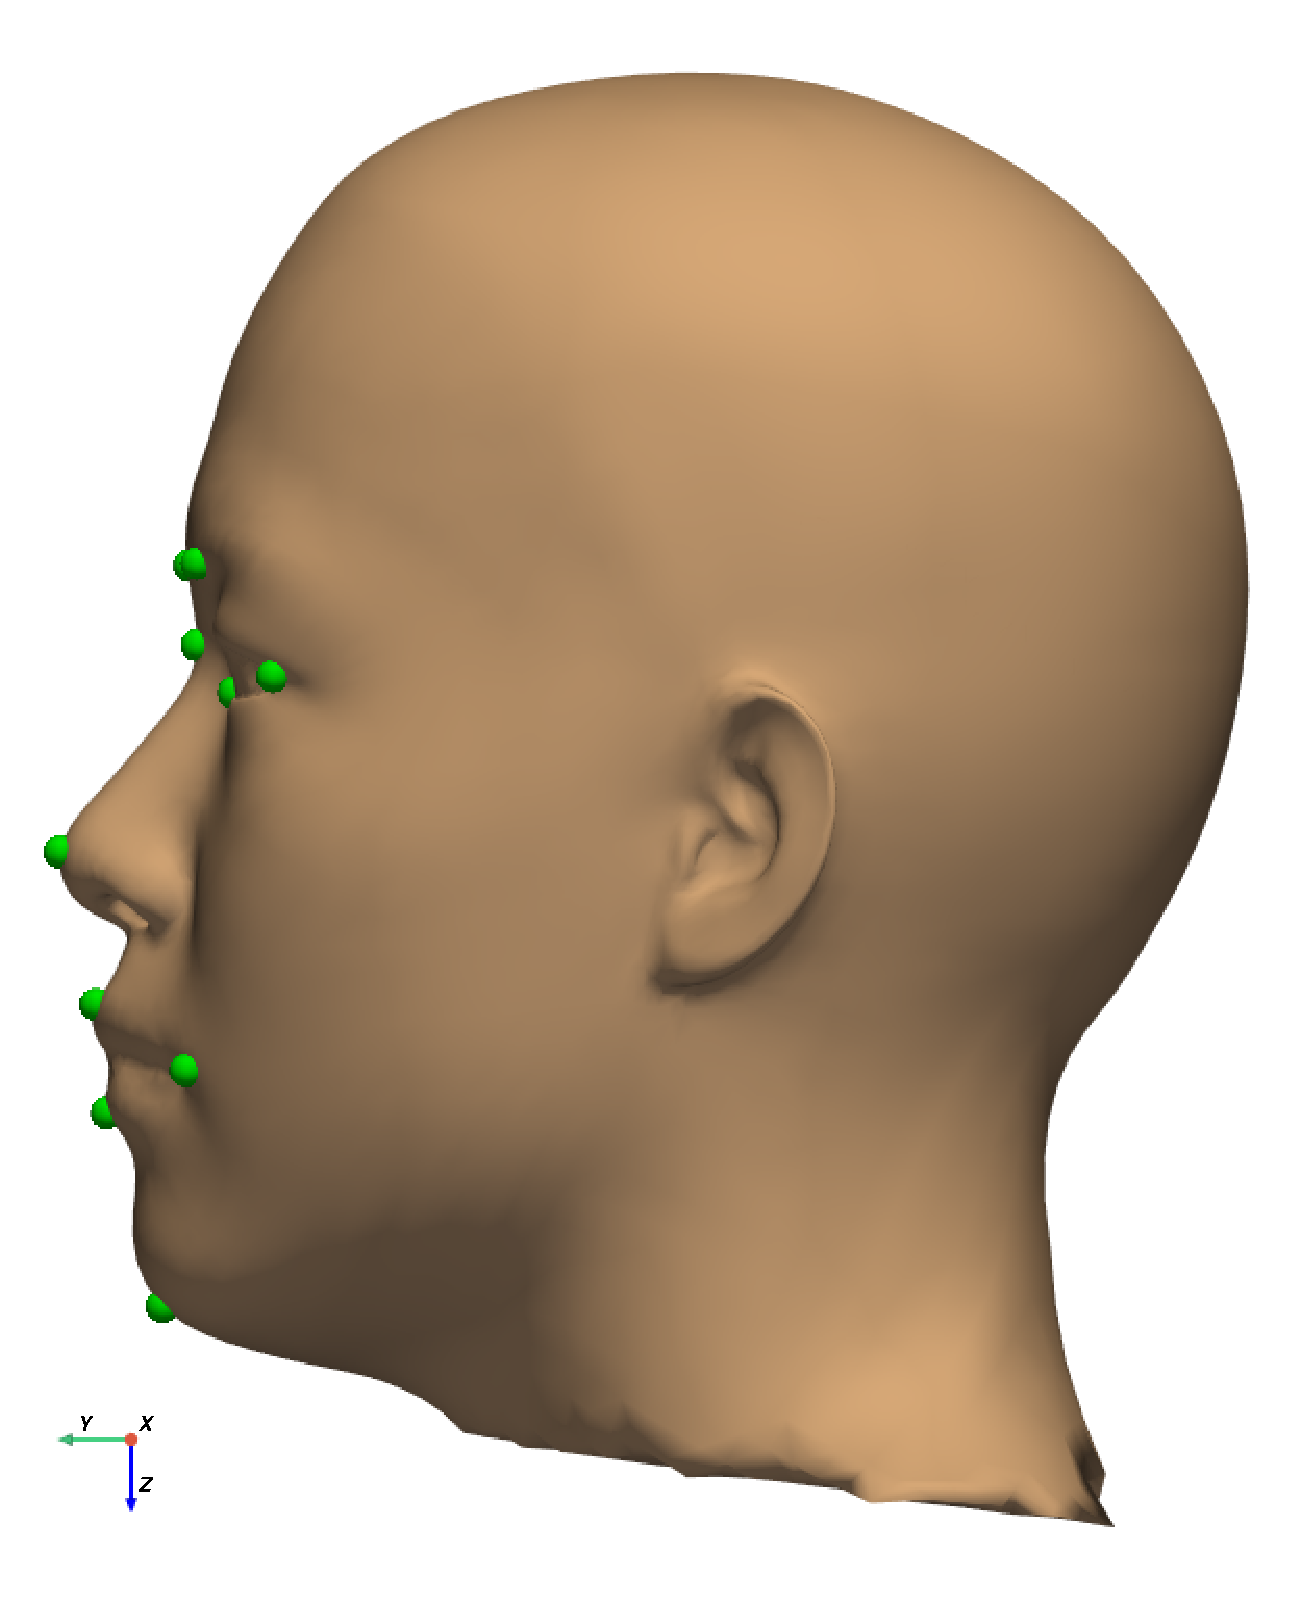
\includegraphics[height = 0.29 \linewidth]{fig/source-face-side.pdf}  & 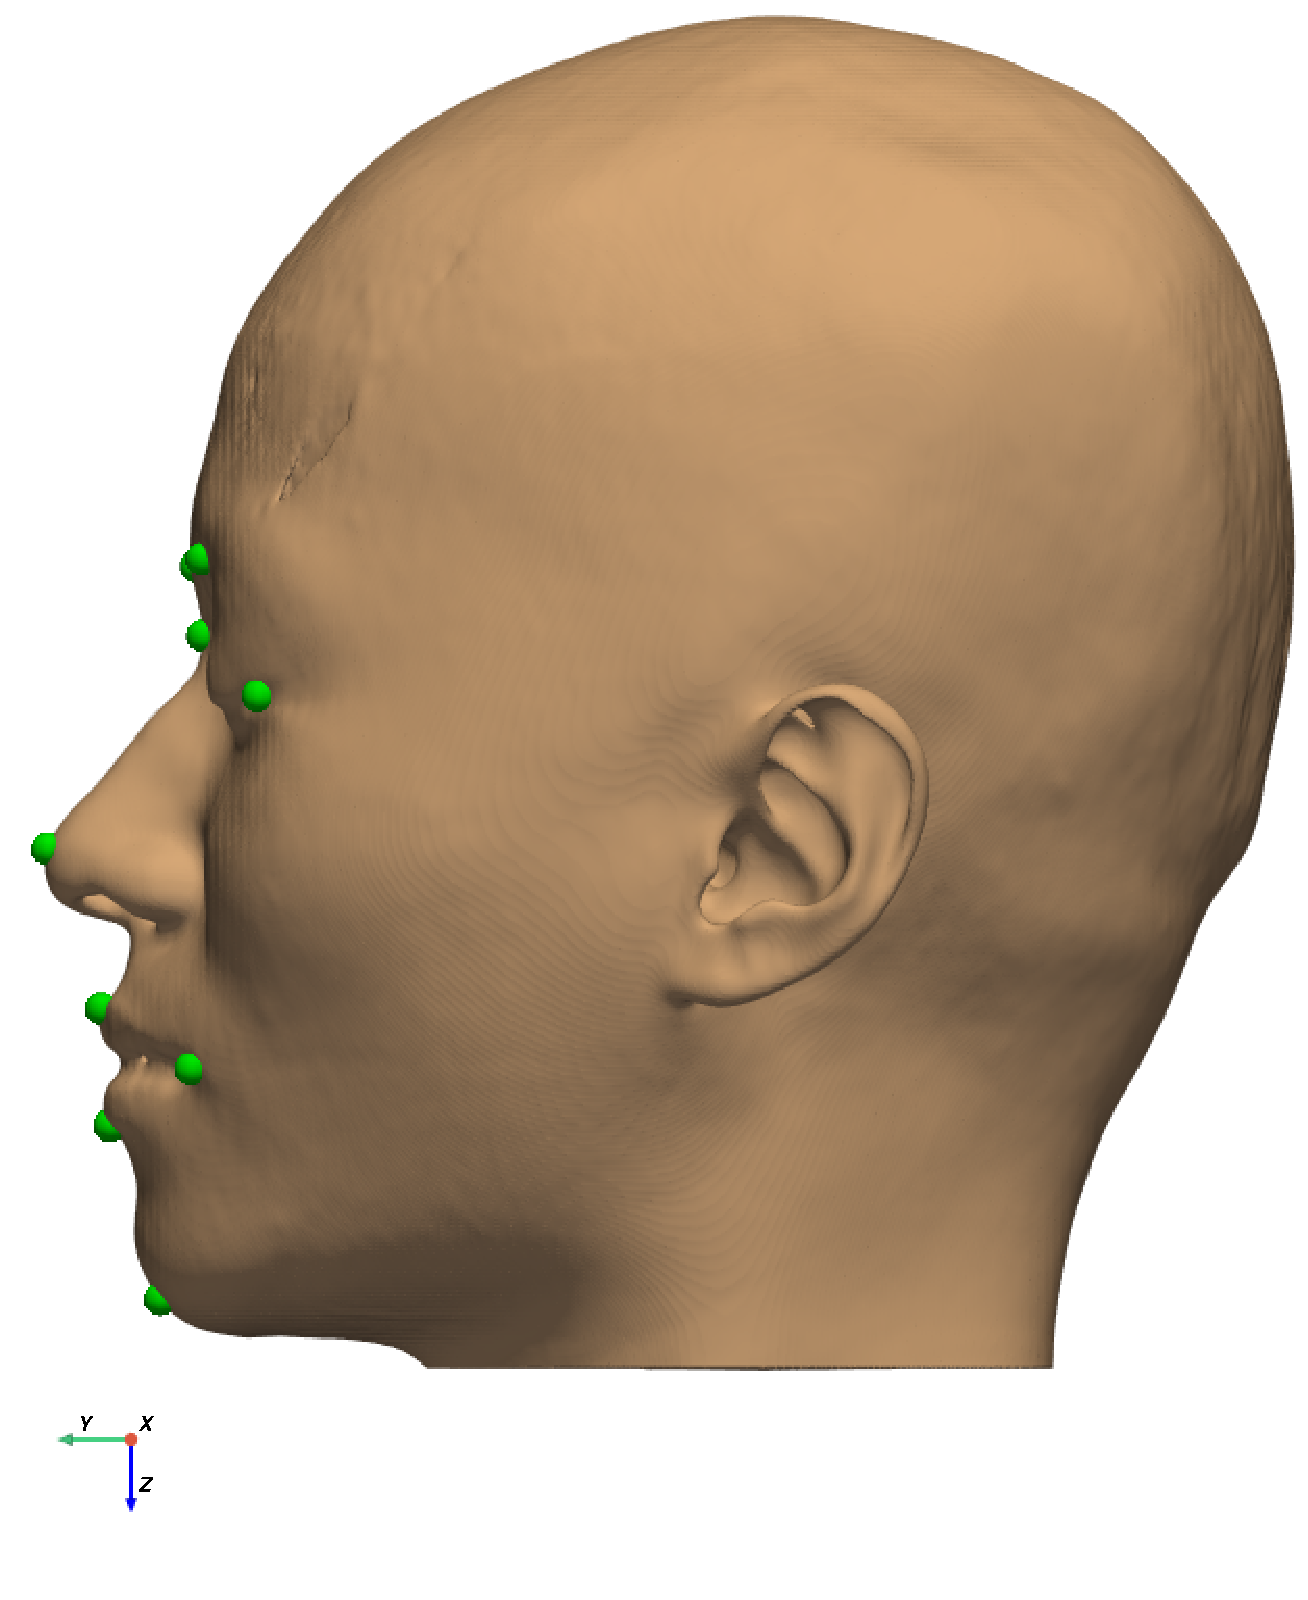
\includegraphics[height = 0.29 \linewidth]{fig/target-face-side.pdf}  & 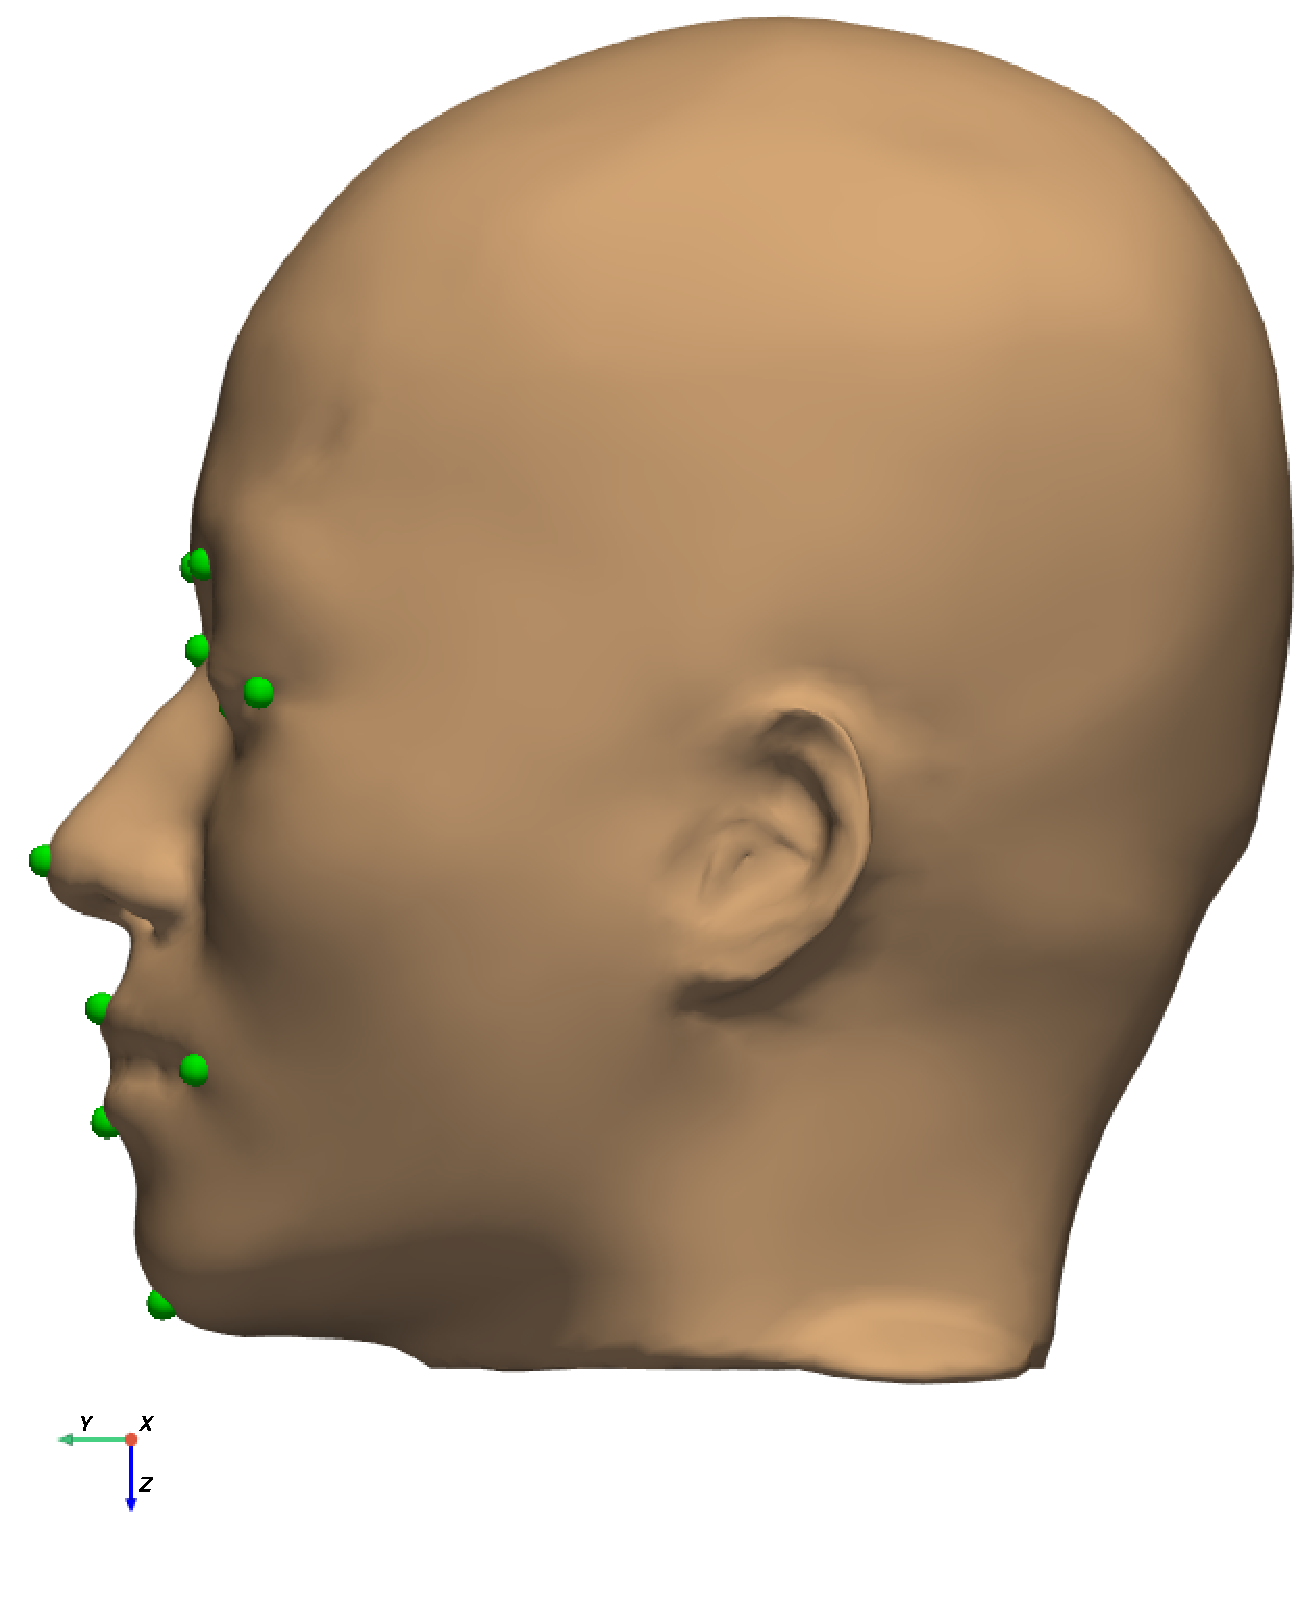
\includegraphics[height = 0.29 \linewidth]{fig/result-face-side.pdf}  \\
    \end{tabular}
  \end{table}
\end{frame}

\begin{frame}{Non-rigid Registration}
  \begin{table}
    \centering
    \begin{tabular}{ccc}
      Template                                                               & Patient                                                                & Result                                                                 \\
      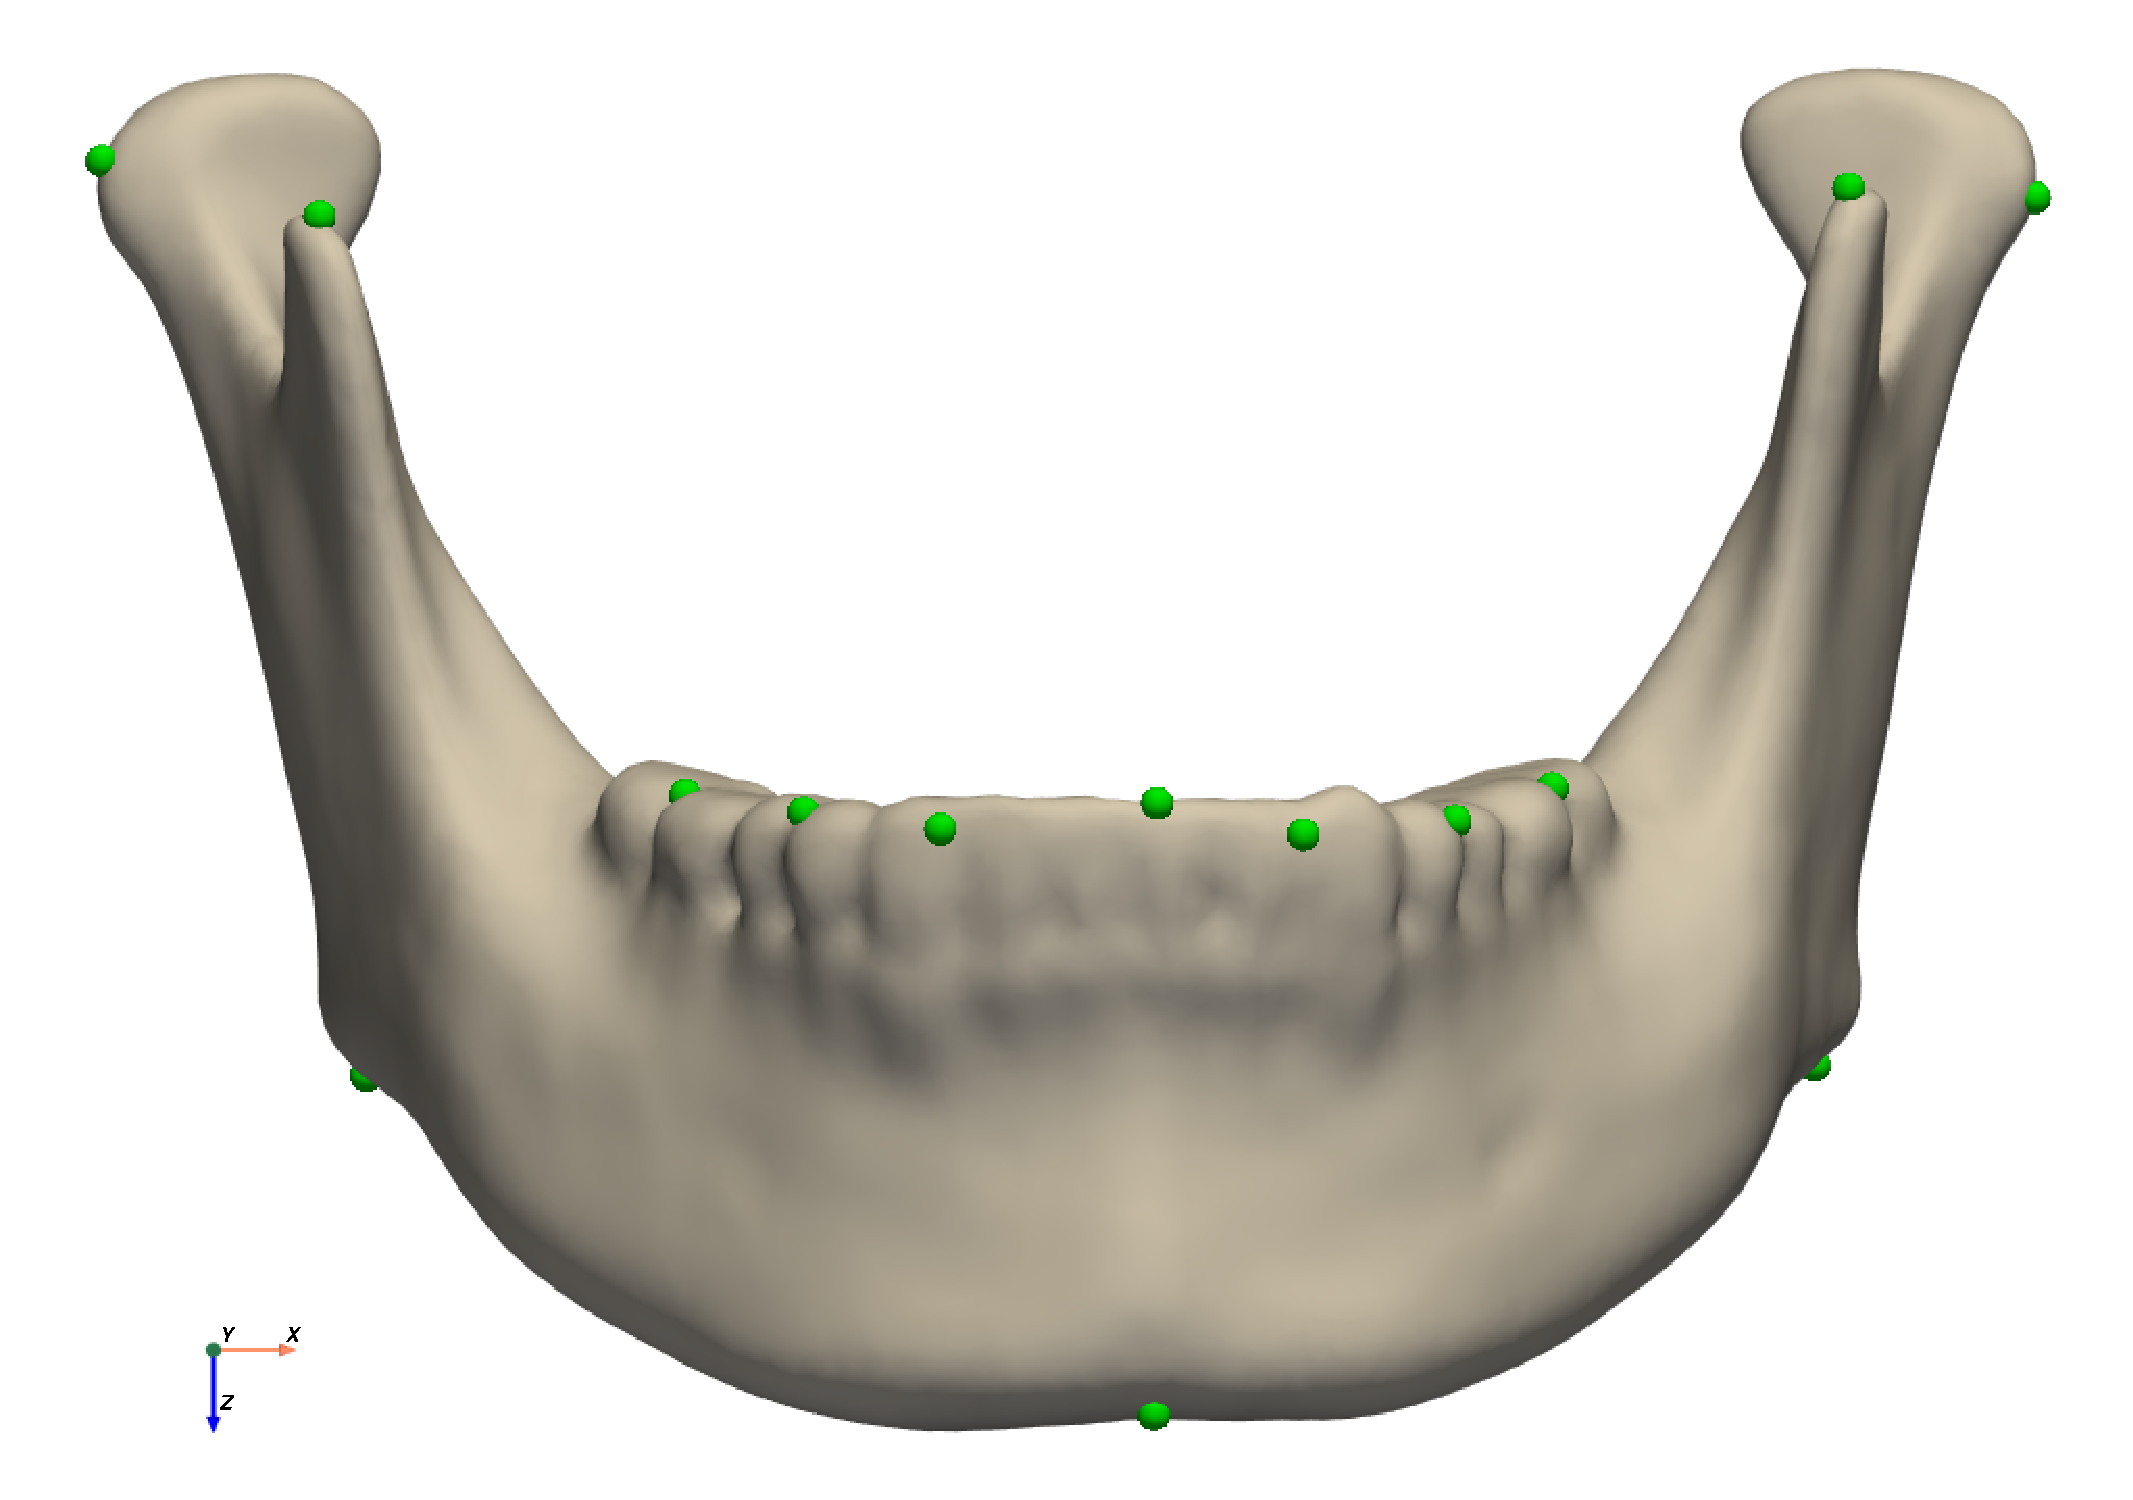
\includegraphics[height = 0.20 \linewidth]{fig/source-skull-front.pdf} & 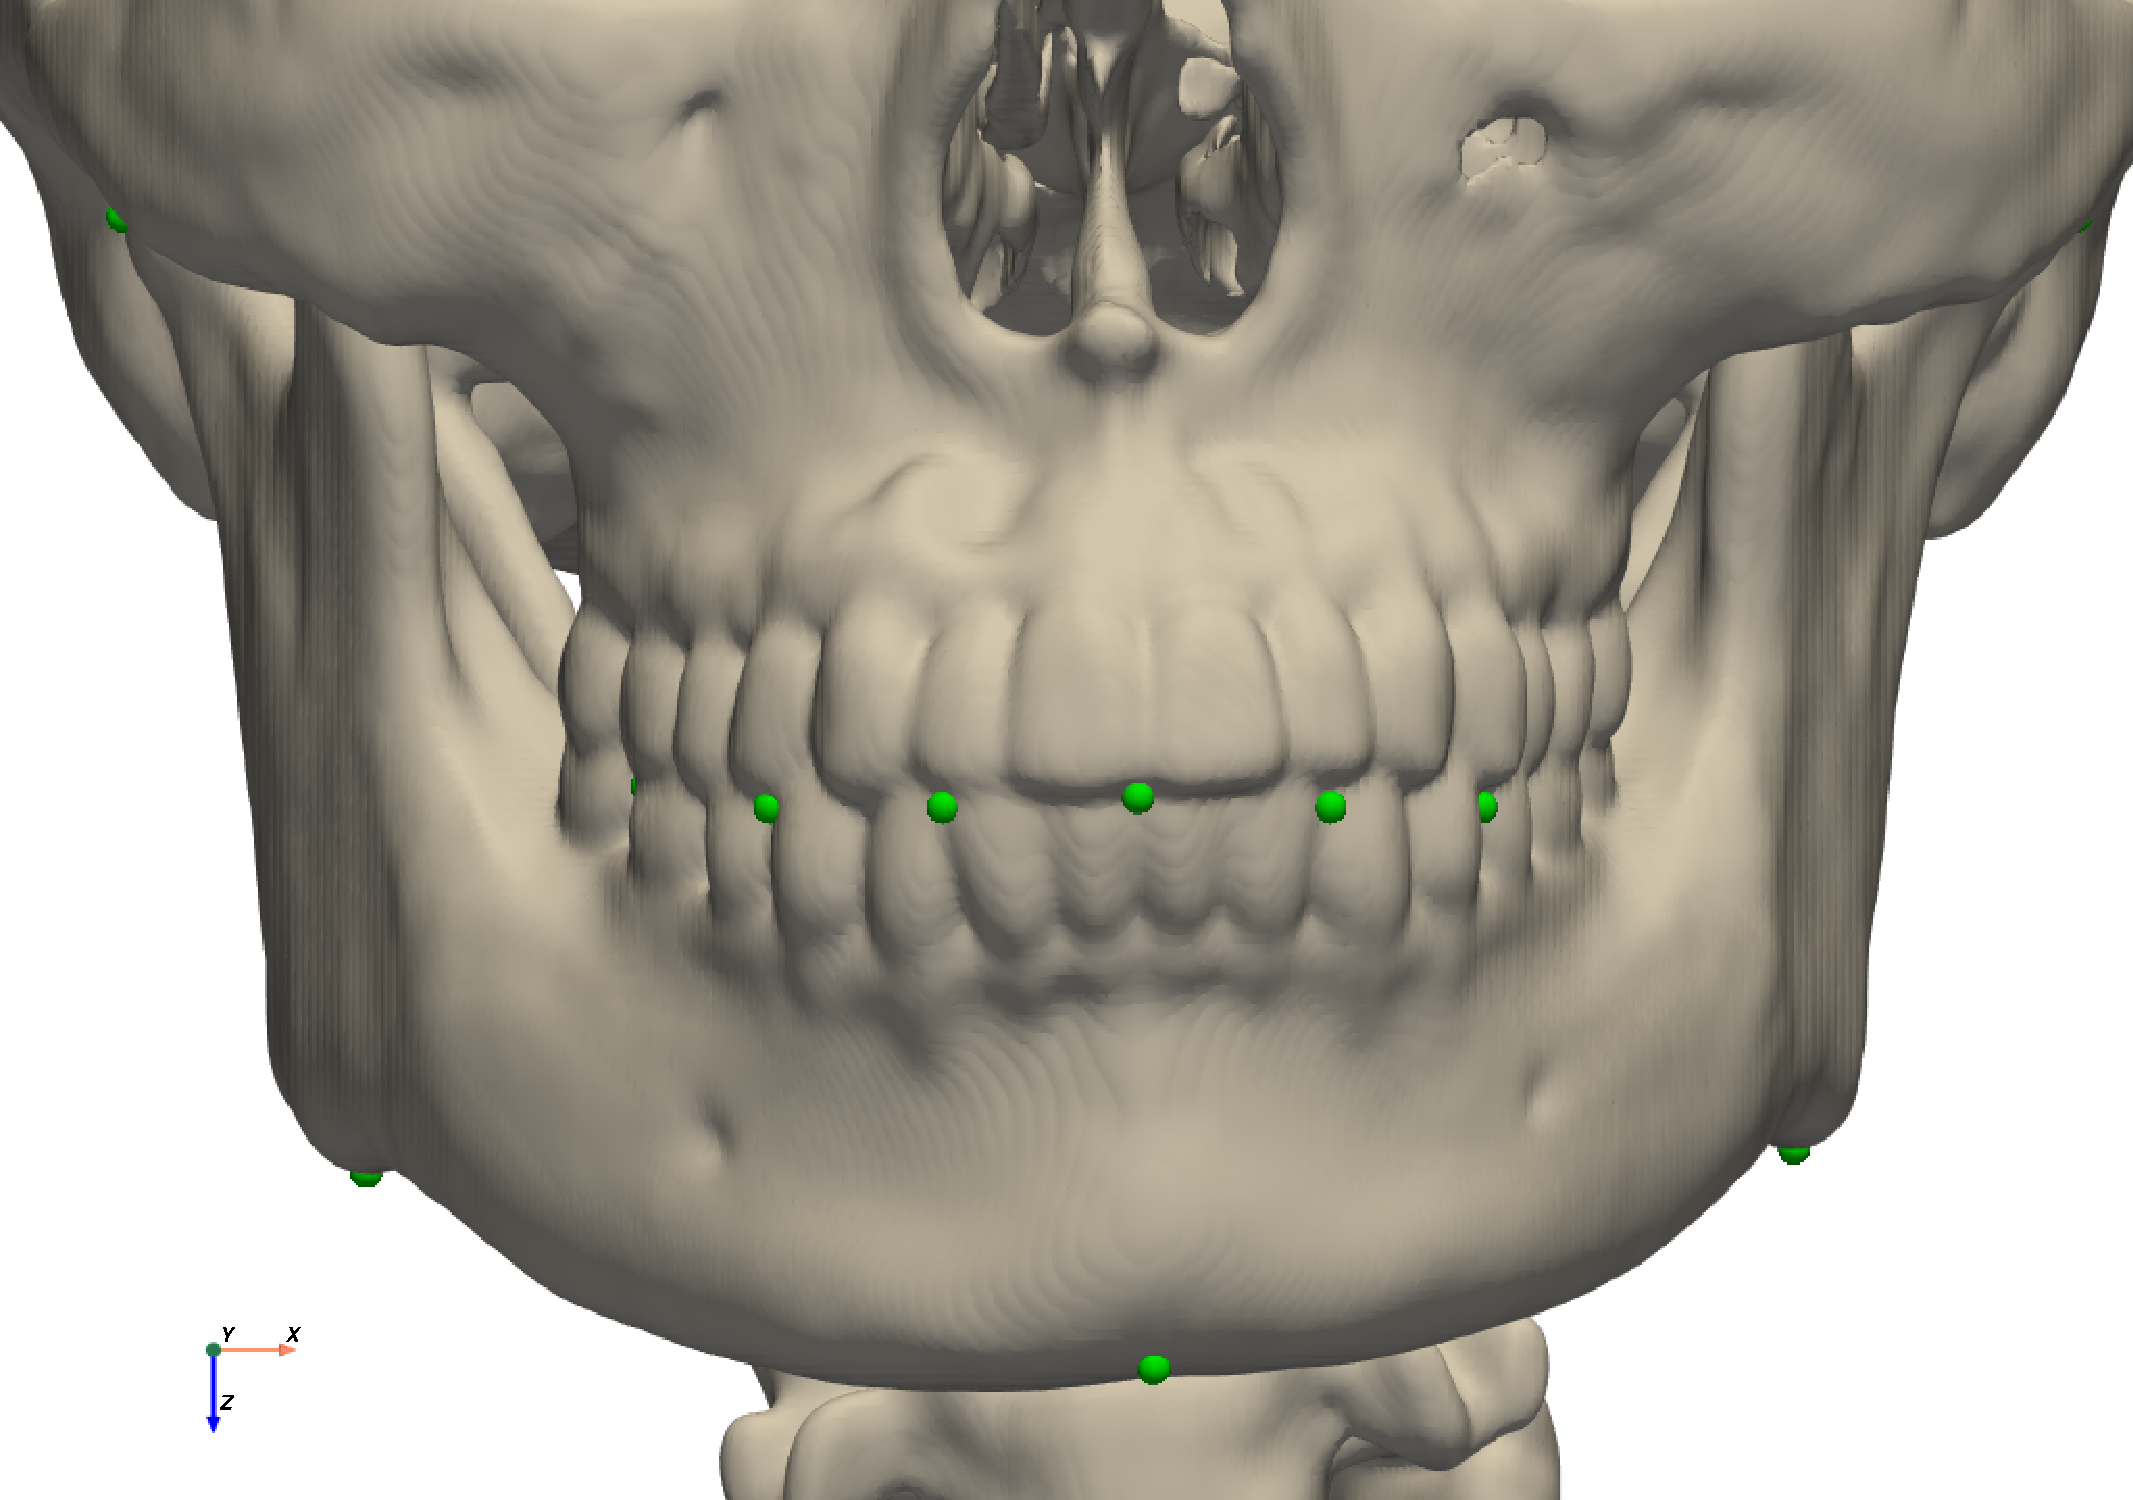
\includegraphics[height = 0.20 \linewidth]{fig/target-skull-front.pdf} & 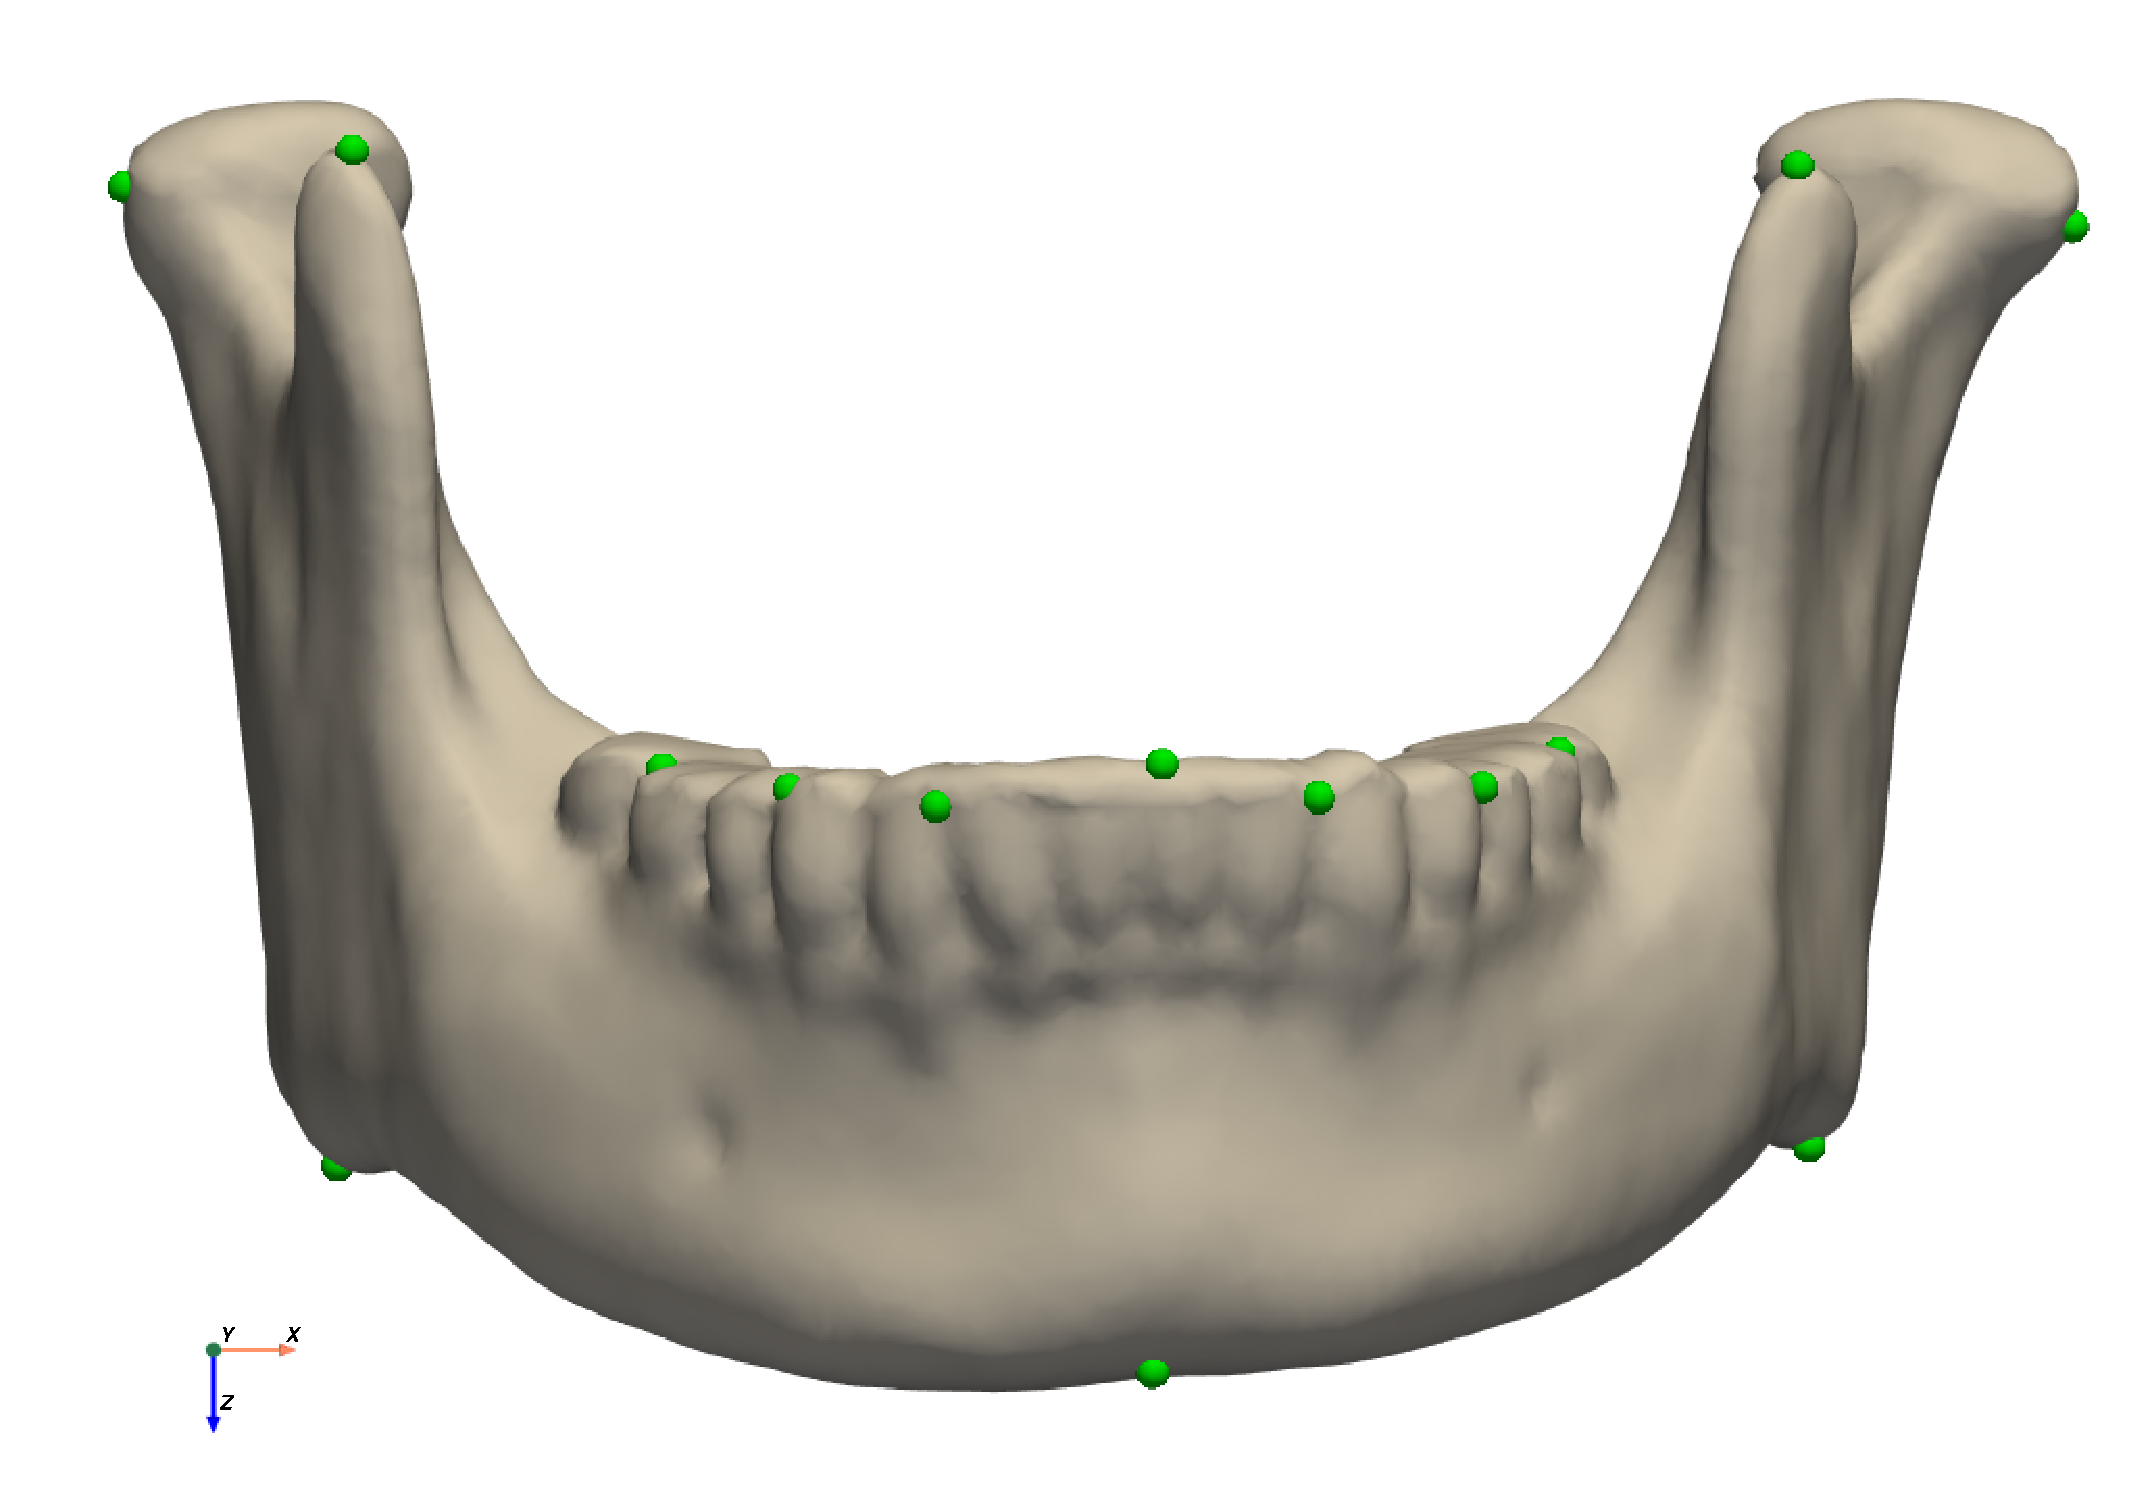
\includegraphics[height = 0.20 \linewidth]{fig/result-skull-front.pdf} \\
      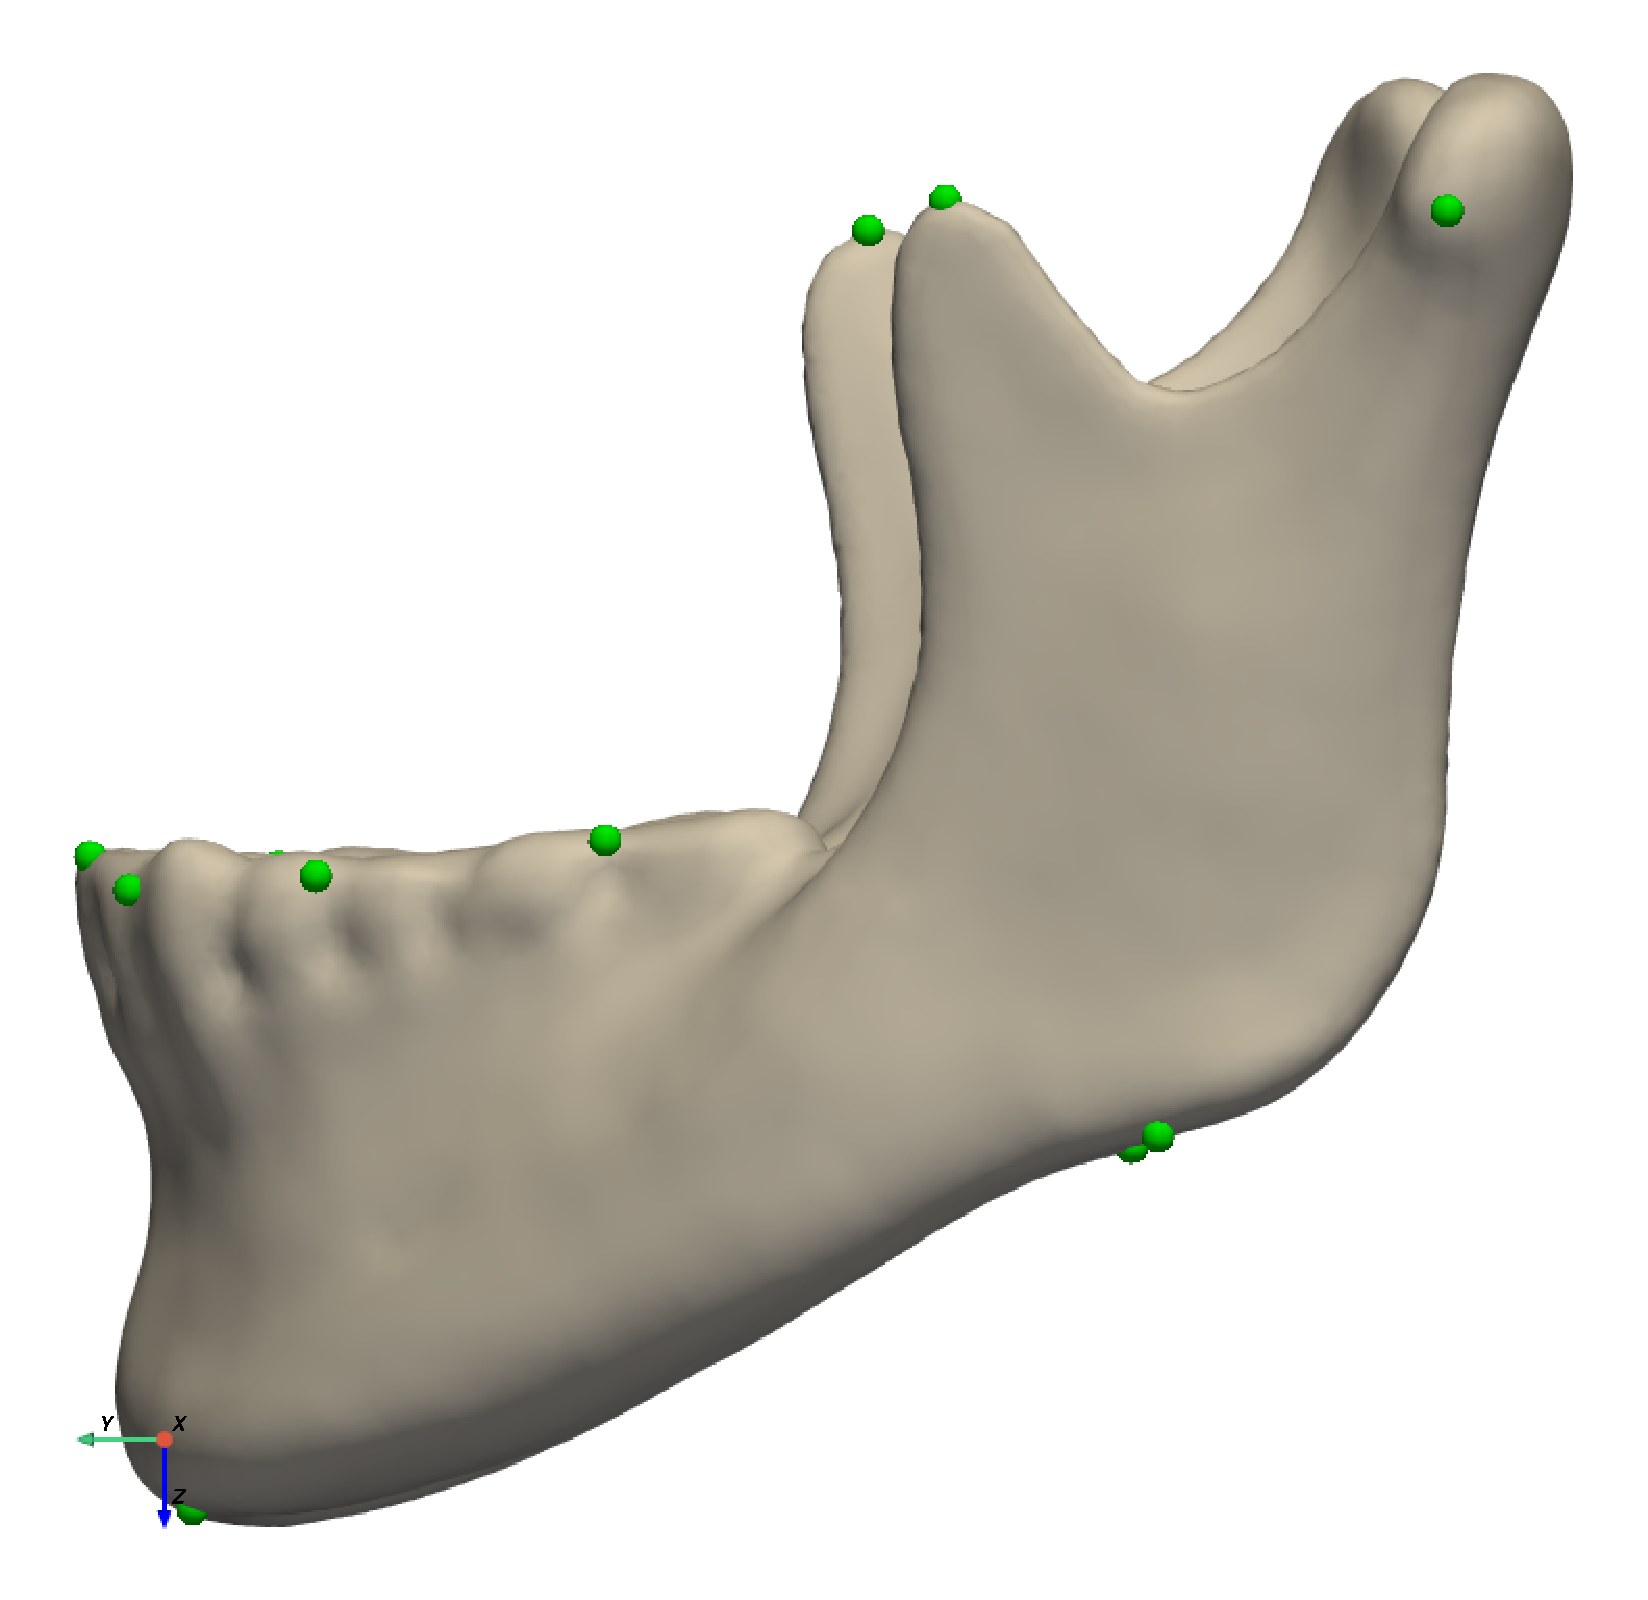
\includegraphics[height = 0.20 \linewidth]{fig/source-skull-side.pdf}  & 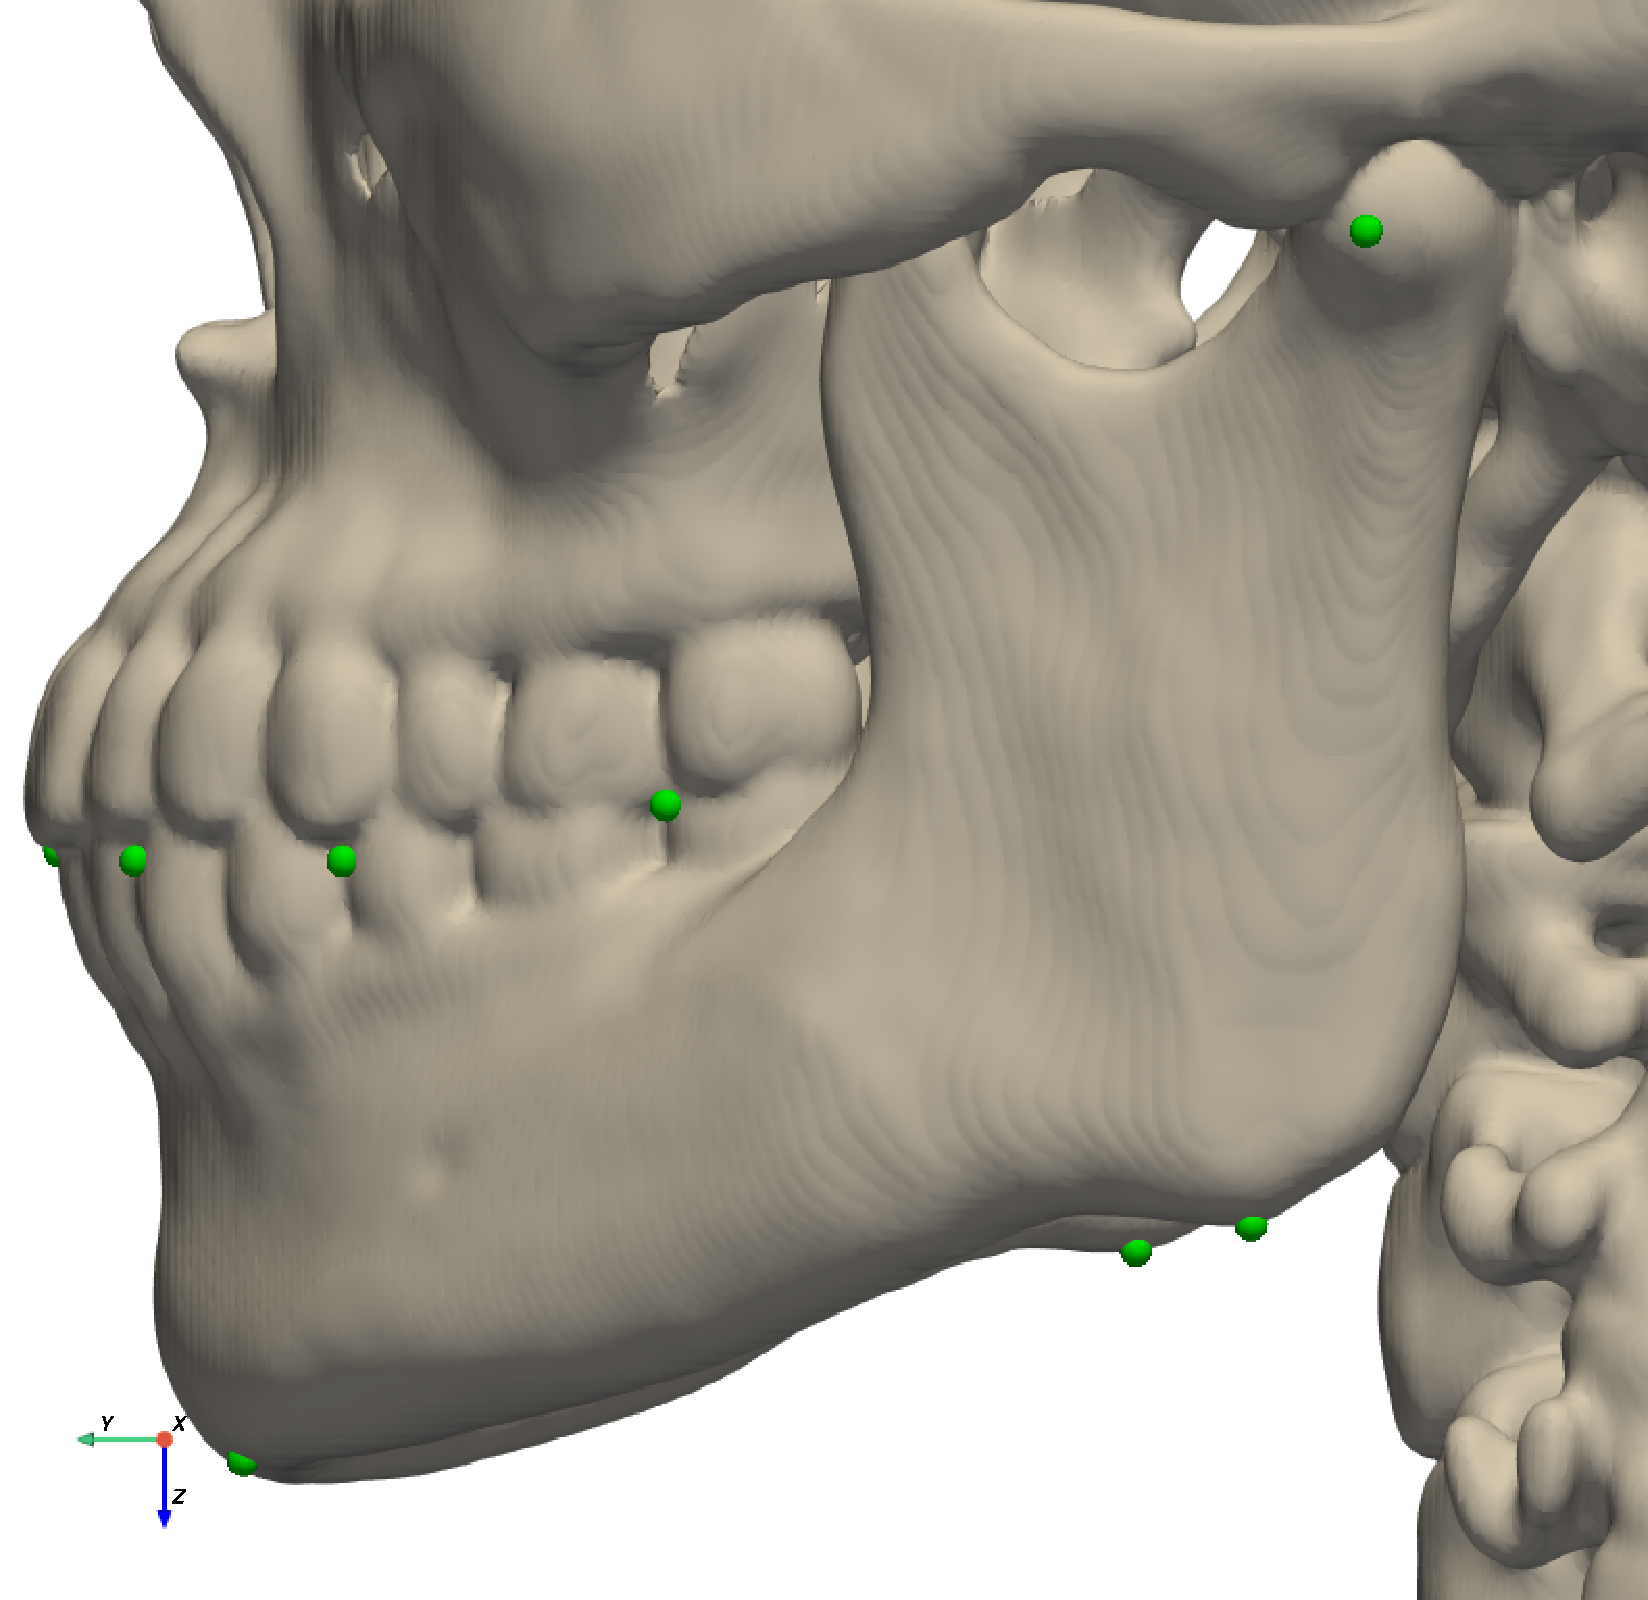
\includegraphics[height = 0.20 \linewidth]{fig/target-skull-side.pdf}  & 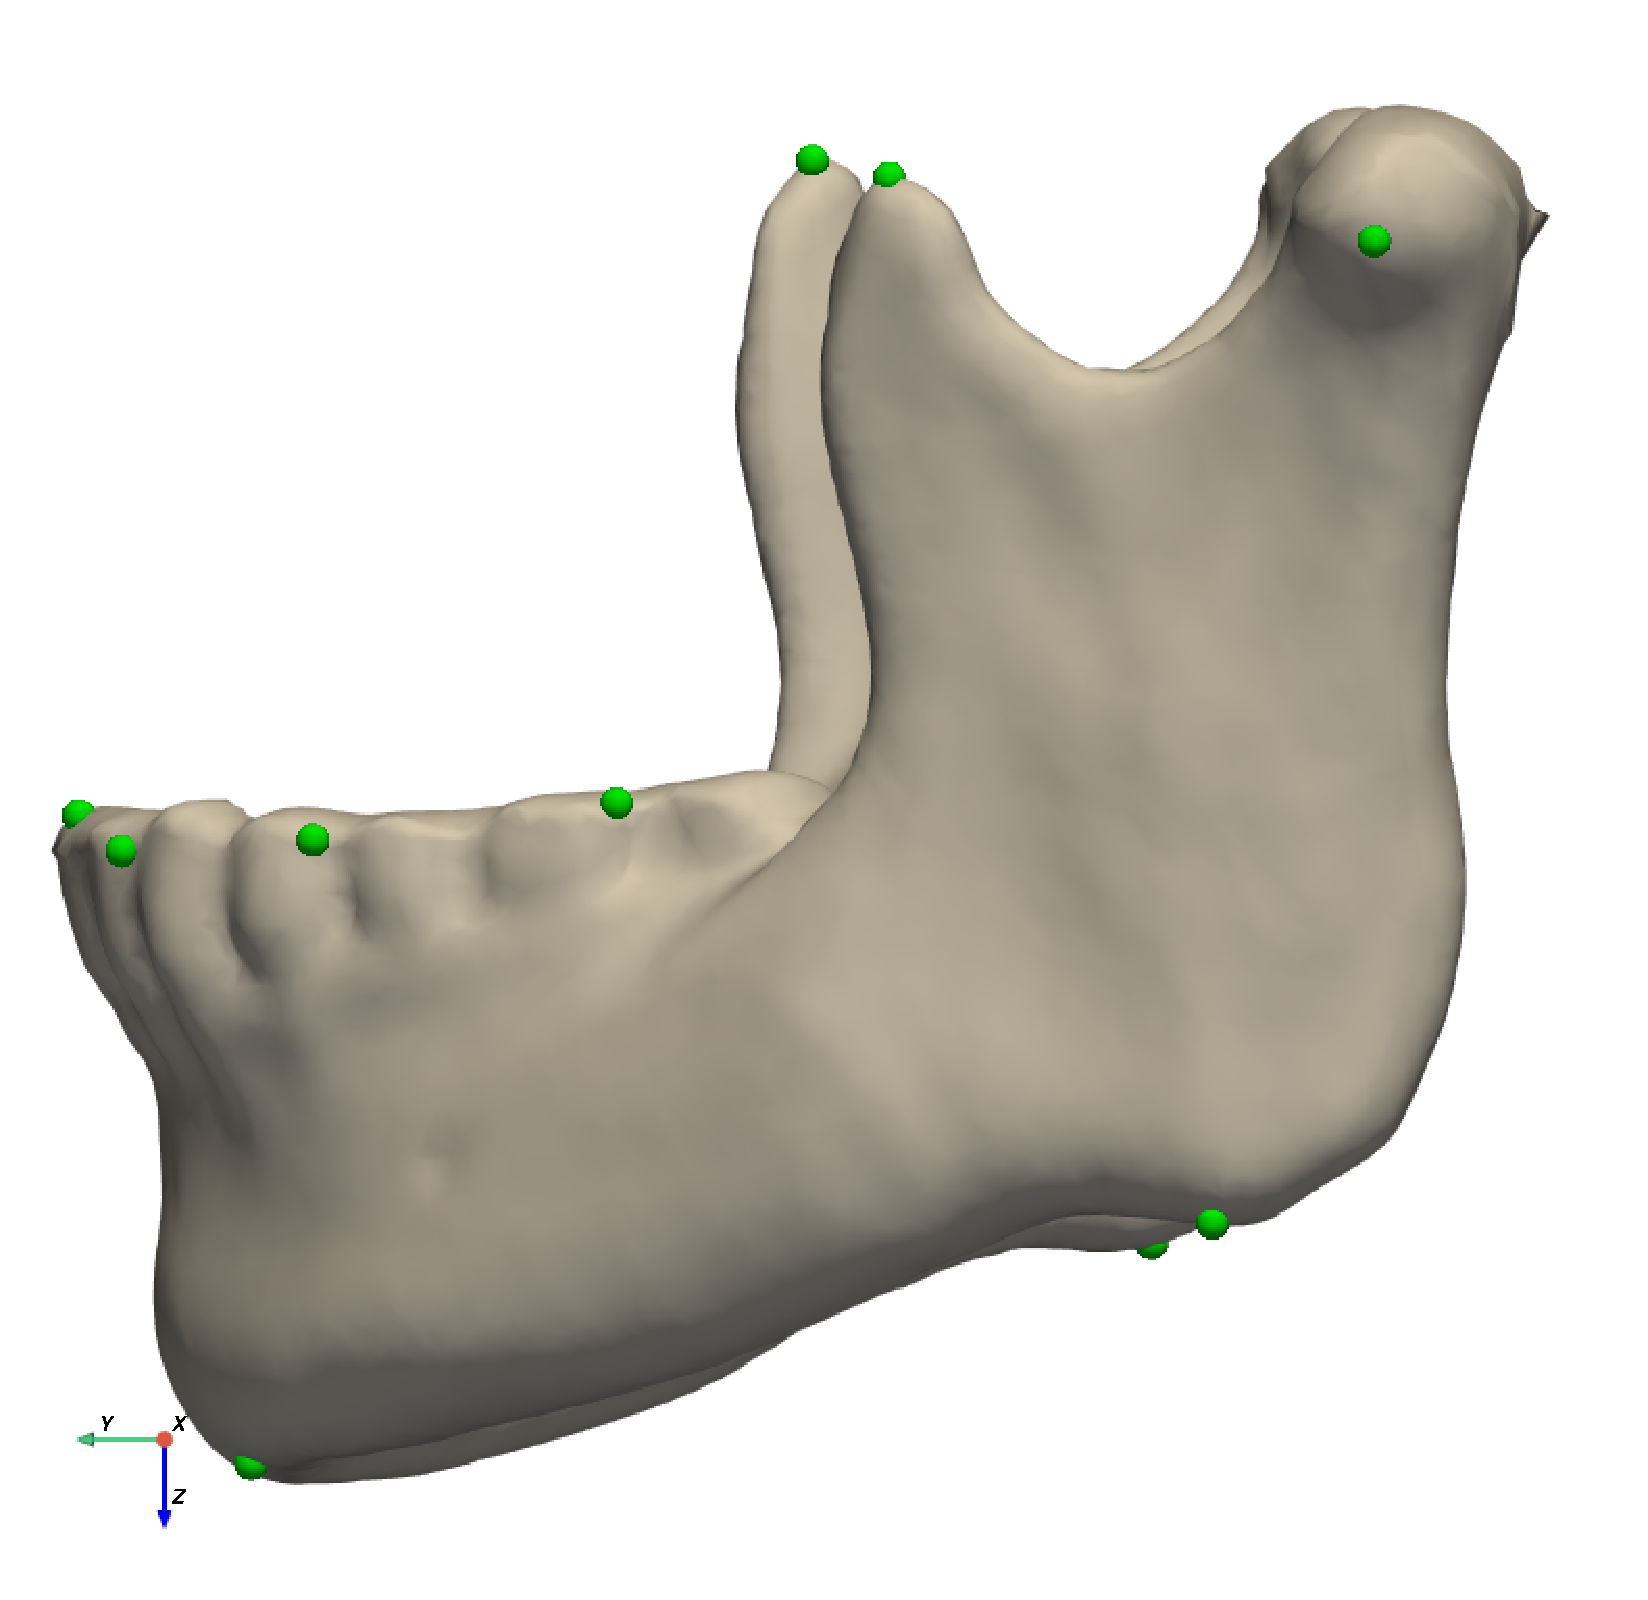
\includegraphics[height = 0.20 \linewidth]{fig/result-skull-side.pdf}  \\
    \end{tabular}
  \end{table}
\end{frame}

\section{Mass-Tensor Model}

\begin{frame}{Mass-Tensor Model}
  \textcolor{tsinghua}{目标} 建模力 $\bm{f}$ 与位移 $\bm{x}$ 之间的关系

  \begin{align*}
    \text{strain tensor} \quad \bm{E} & = \frac{1}{2} (\nabla U + \nabla U^T)                     \\
    \text{elastic energy} \quad W     & = \frac{1}{2} \lambda (\tr(\bm{E}))^2 + \mu \tr(\bm{E}^2) \\
    \text{nodal force} \quad \bm{f}_i & = \pdv{W}{\bm{p}_i} \Rightarrow \bm{f} = \bm{K} \bm{x}
  \end{align*}
  \begin{align*}
    \bm{f}_i          & = \bm{K}_{ii} \bm{x}_i + \sum_{\bm{v}_j \in N(\bm{v}_i)} \bm{K}_{ij} \bm{x}_j                                                    \\
    \bm{K}_{ij}^{T_i} & = \frac{1}{36 V} (\lambda \bm{M}_k \bm{M}_j^T + \mu \bm{M}_j \bm{M}_k^T + \mu (\bm{M}_j \bm{M}_k) \bm{I})                        \\
    \pm \bm{M}_j      & = \bm{p}_{j + 1}^0 \times \bm{p}_{j + 2}^0 + \bm{p}_{j + 2}^0 \times \bm{p}_{j + 3}^0 + \bm{p}_{j + 3}^0 \times \bm{p}_{j + 1}^0
  \end{align*}
\end{frame}

\begin{frame}{Mass-Tensor Model}
  \begin{equation*}
    \begin{bmatrix}
      K_{00} & K_{01} \\
      K_{10} & K_{11}
    \end{bmatrix}
    \begin{bmatrix}
      x_0 \\
      x_1
    \end{bmatrix}
    =
    \begin{bmatrix}
      f_0 \\
      f_1
    \end{bmatrix}
  \end{equation*}
  \begin{description}
    \item[$K$] stiffness matrix
    \item[$f$] external force
    \item[$x_0$] 固定的与 skull 紧邻的点的位移
    \item[$x_1$] 待求解的自由点位移 (包括 face 上的点和填充的点)
  \end{description}
  令 $f_1 = 0$ 可得
  \begin{equation*}
    K_{01} x_0 + K_{11} x_1 = f_1 = 0
  \end{equation*}
  $K_{11}$ 并不保证正定, 因此使用 MINRES 求解
\end{frame}

\begin{frame}{Simulation Results}
  \begin{table}
    \centering
    \begin{tabular}{ccc}
      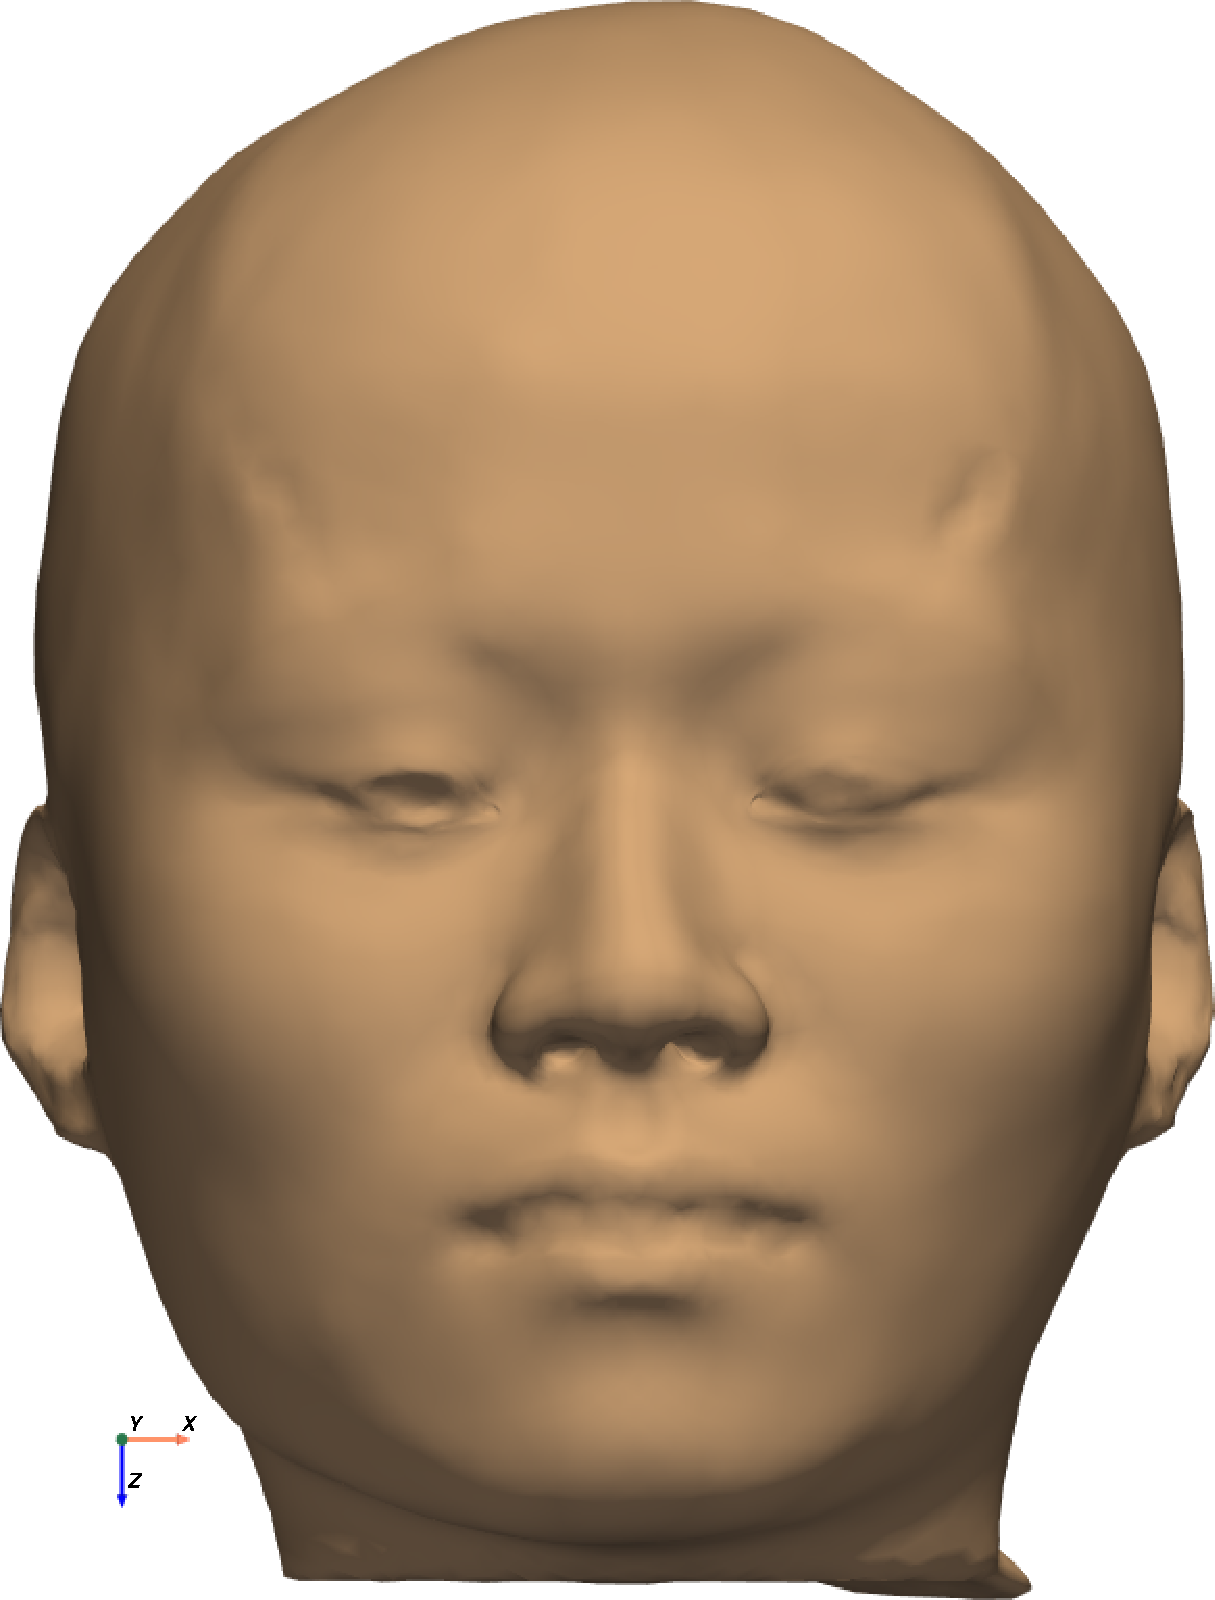
\includegraphics[height = 0.30 \linewidth]{fig/pre-face-front.pdf}  & 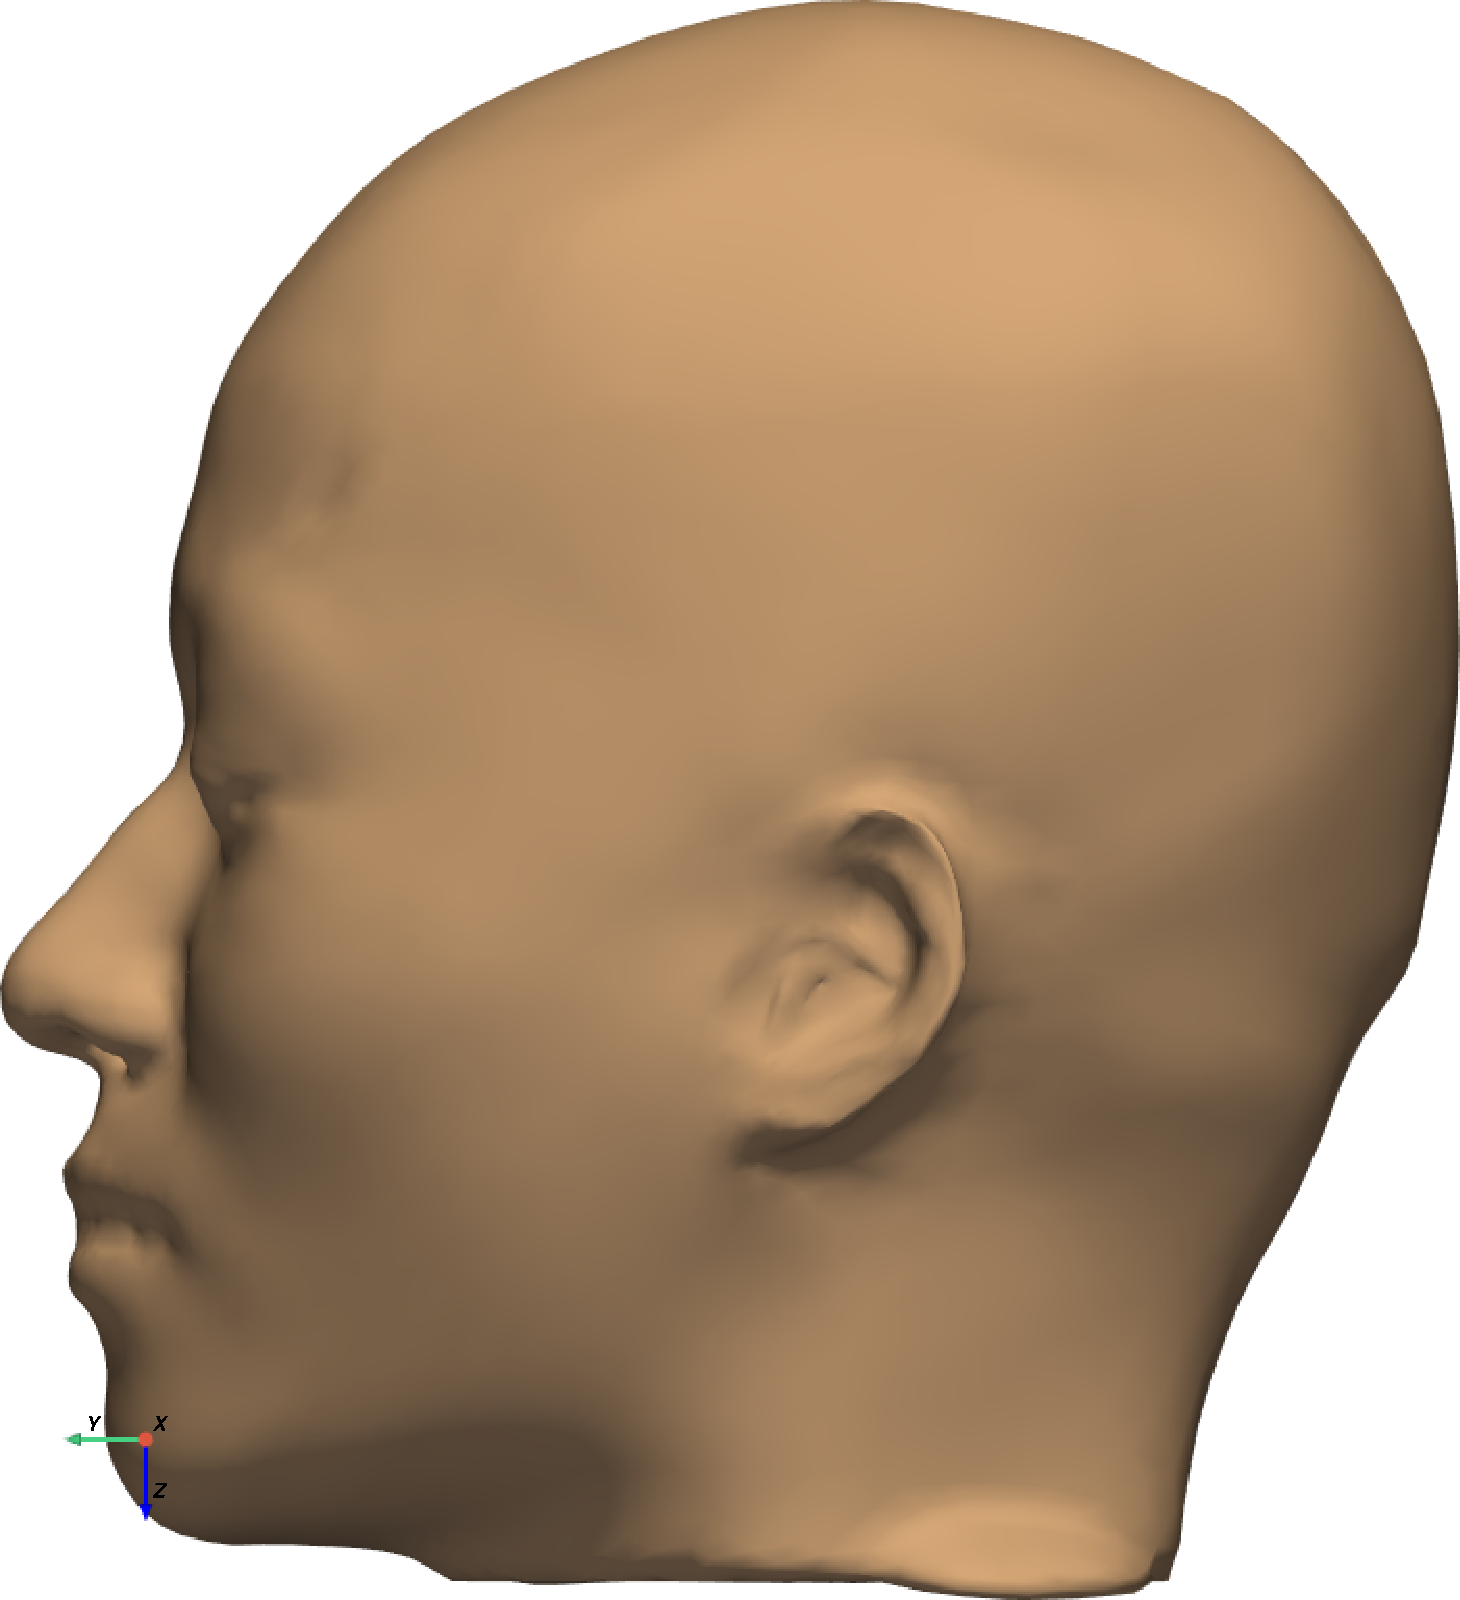
\includegraphics[height = 0.30 \linewidth]{fig/pre-face-side.pdf}  & 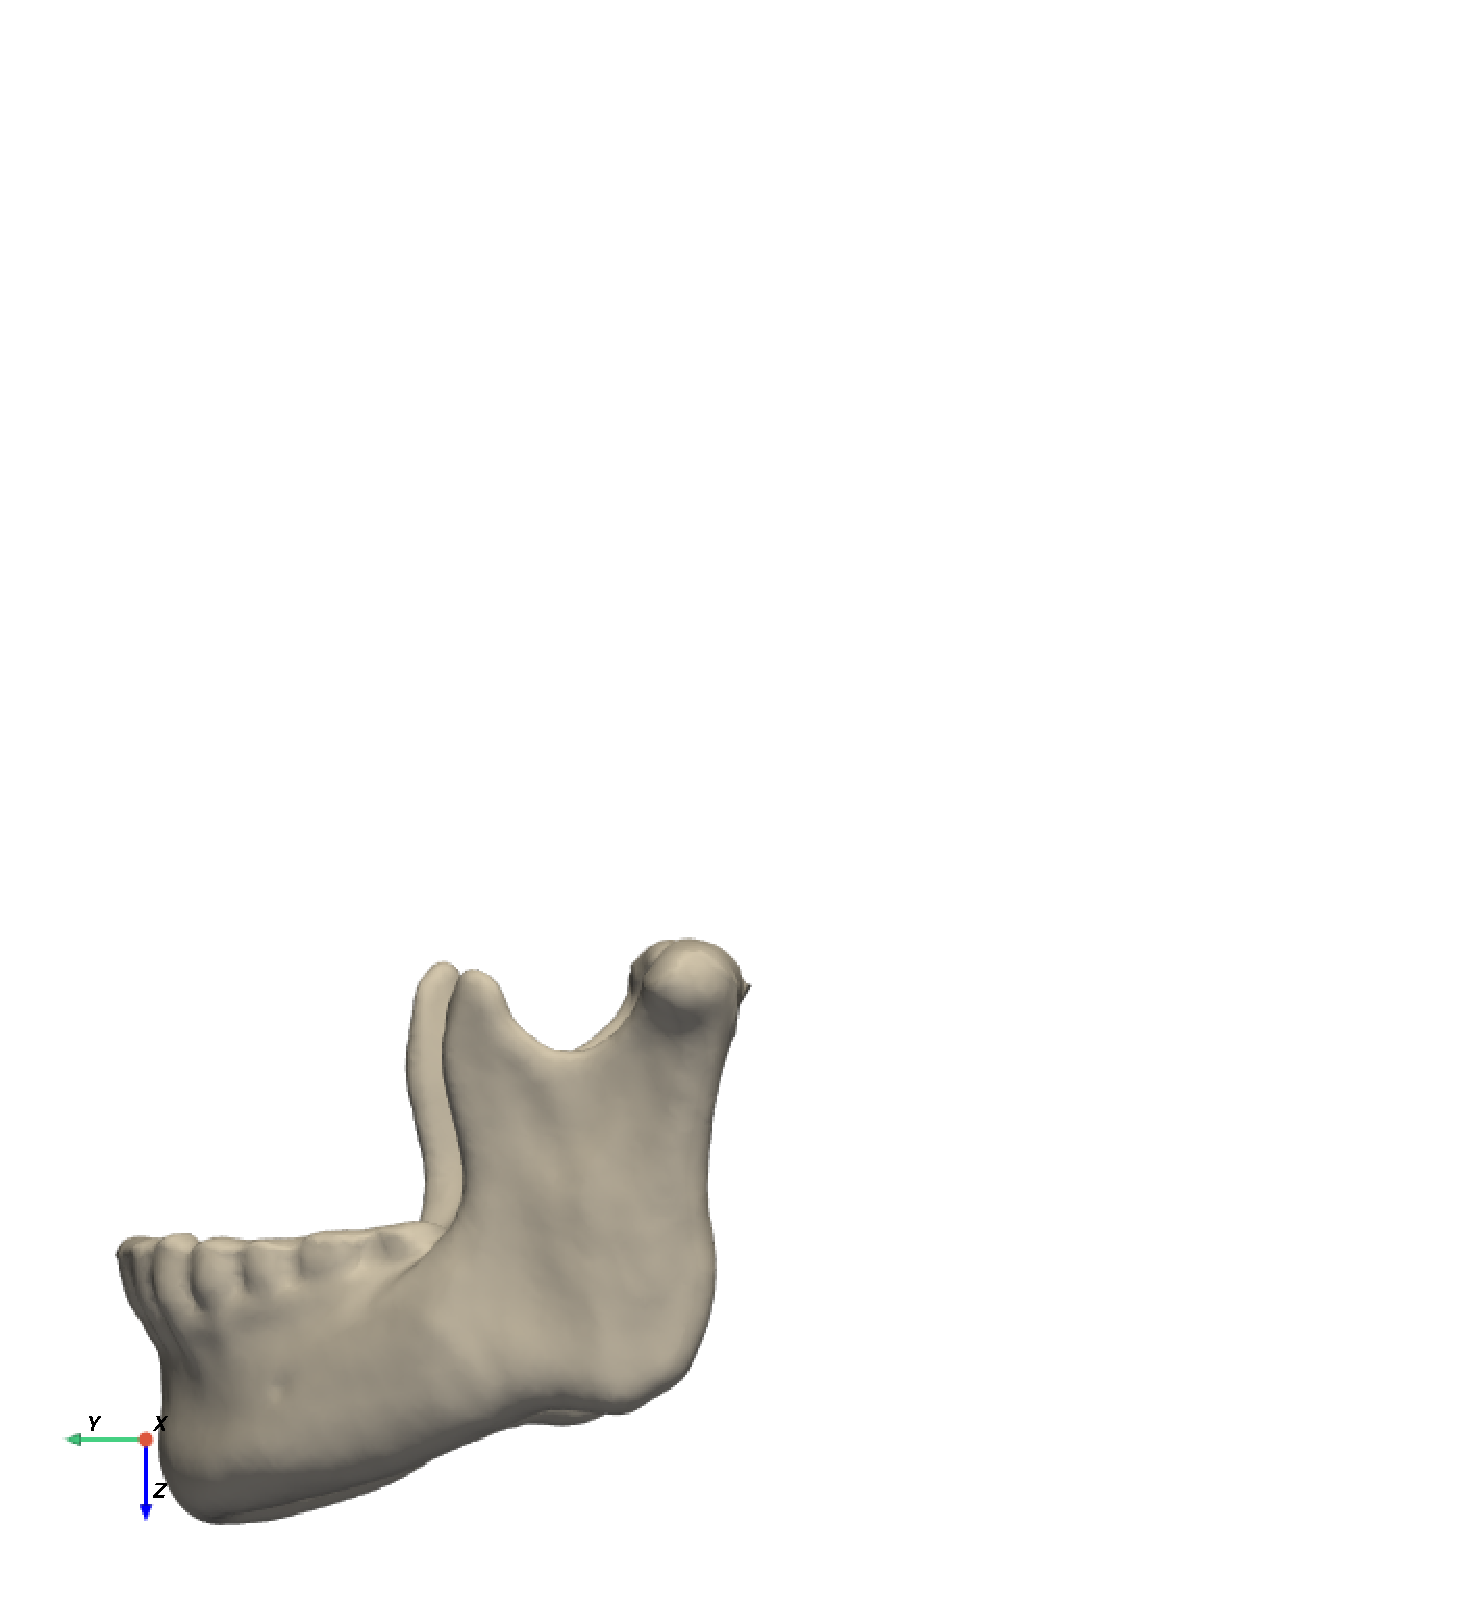
\includegraphics[height = 0.30 \linewidth]{fig/pre-skull-side.pdf}  \\
      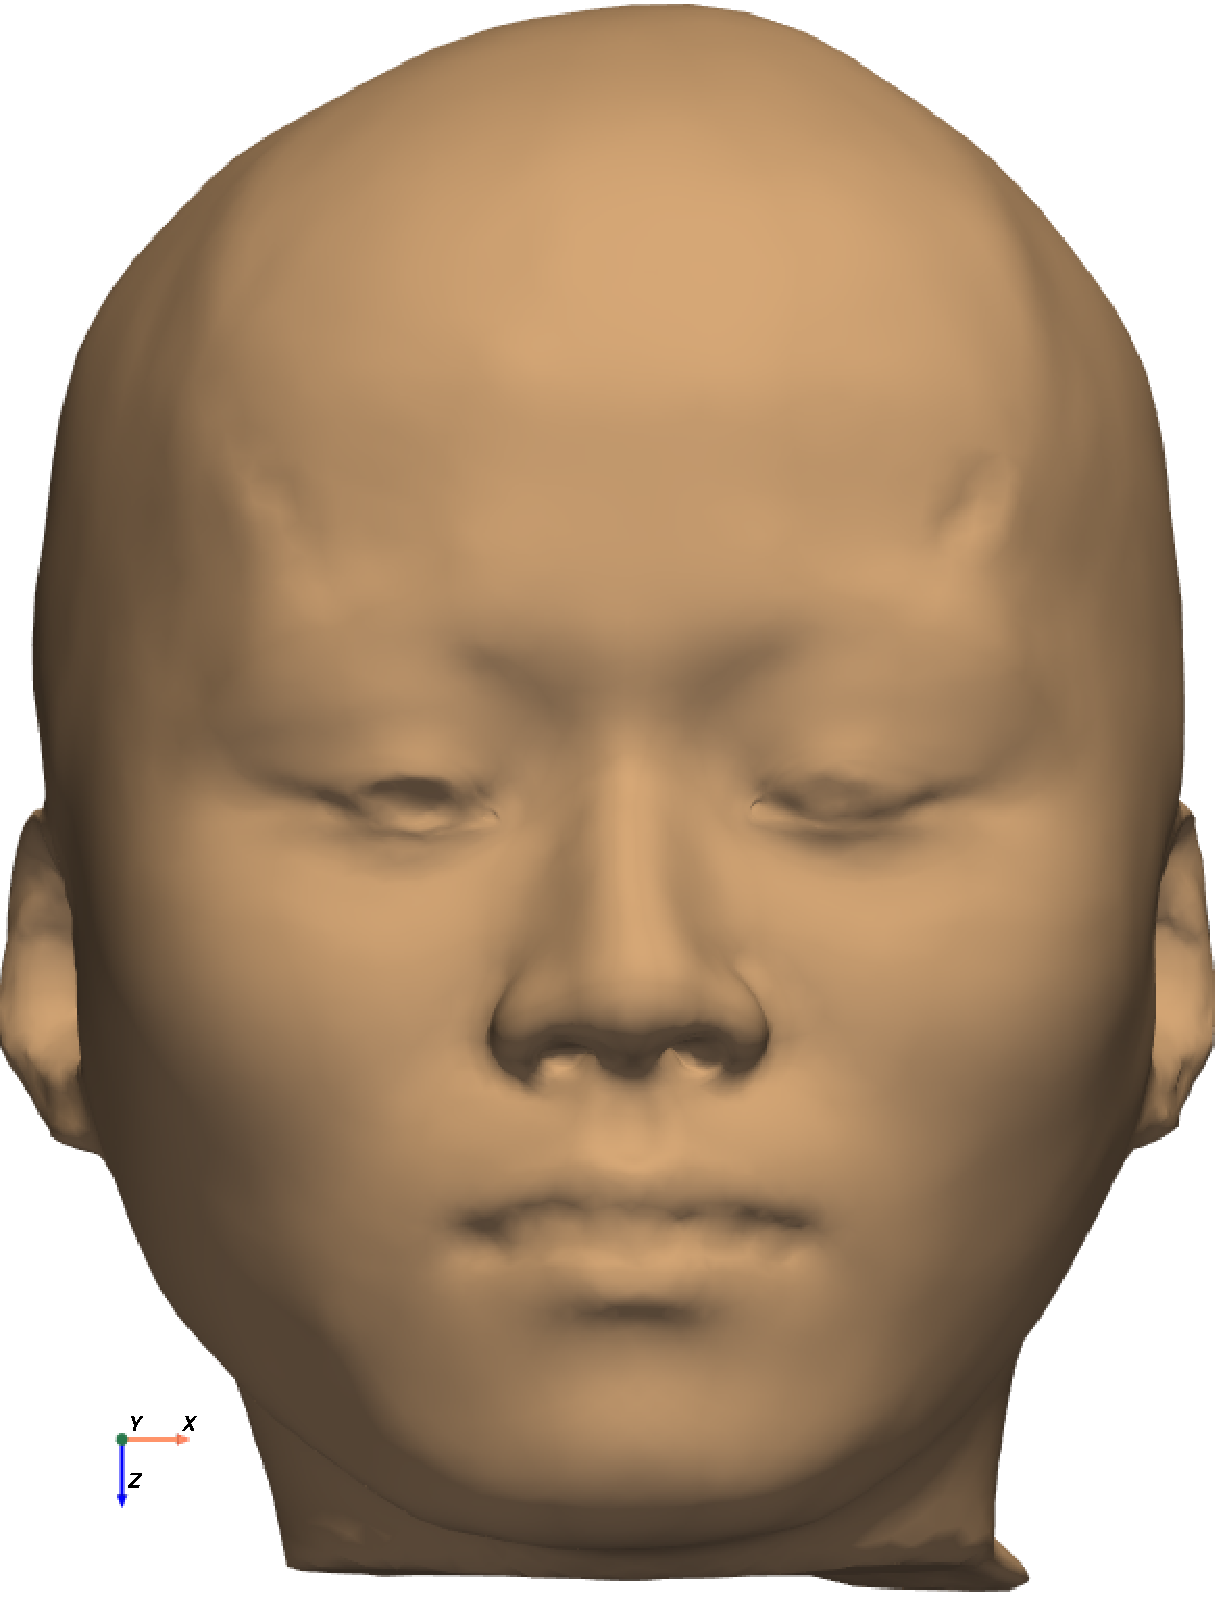
\includegraphics[height = 0.30 \linewidth]{fig/post-face-front.pdf} & 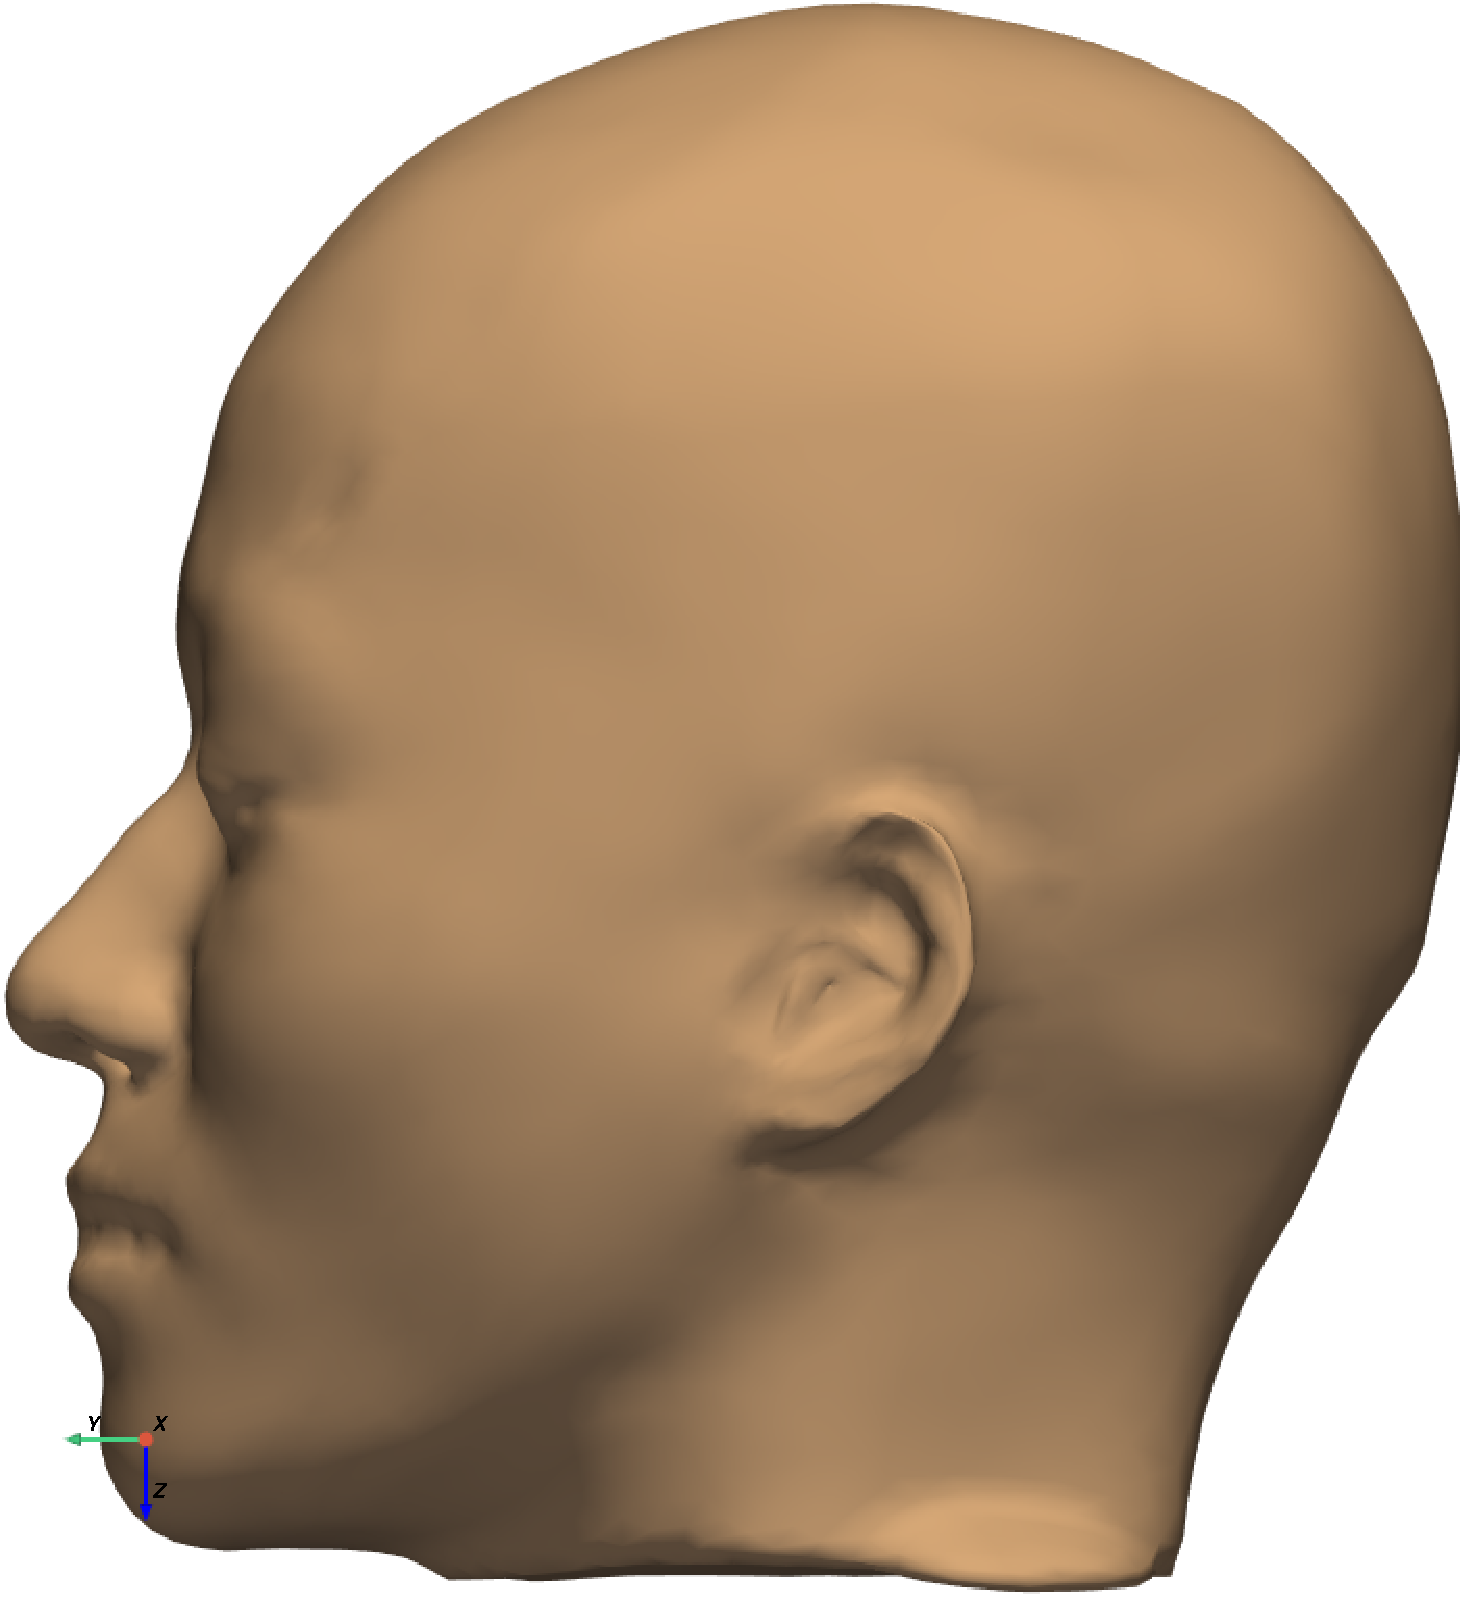
\includegraphics[height = 0.30 \linewidth]{fig/post-face-side.pdf} & 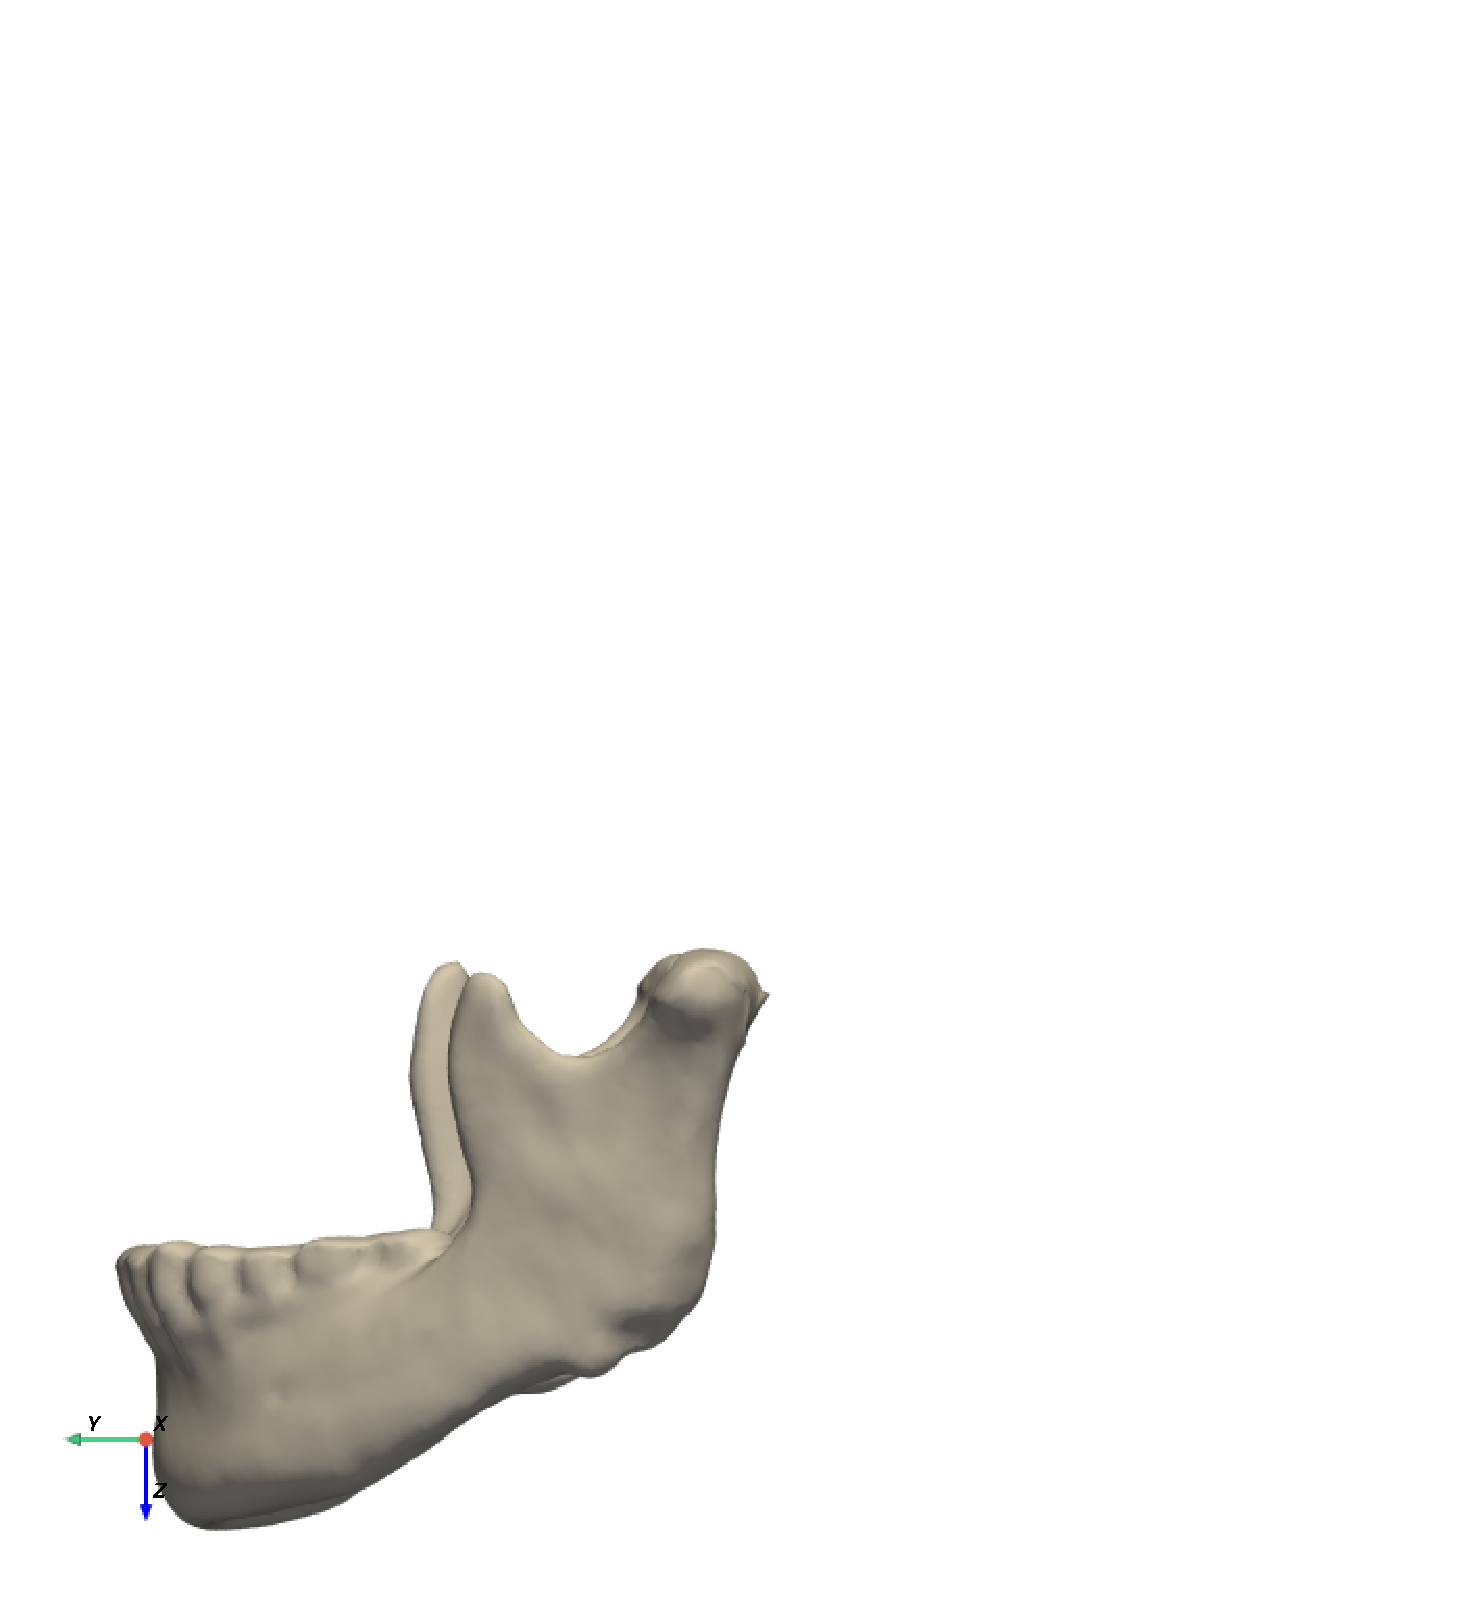
\includegraphics[height = 0.30 \linewidth]{fig/post-skull-side.pdf}
    \end{tabular}
  \end{table}
\end{frame}

\section{TODO}

\begin{frame}{TODO}
  \begin{itemize}
    \item 优化全流程的自动化程度
    \item 优化物理模拟的超参数和鲁棒性
    \item 与真实数据进行对比, 评估准确性
    \item 完成论文的撰写
  \end{itemize}
\end{frame}

\begin{frame}
  \begin{center}
    \Huge
    感谢各位老师的聆听!

    敬请批评指正!
  \end{center}
\end{frame}

\end{document}
